%%%%%%%%%%%%%%%%%%%%%%%%%%%%%%%%%%%%%%%%%%%%%%%%%%
%% Bachelor's & Master's Thesis Template        %%
%% Copyleft by Dawid Weiss & Marta Szachniuk    %%
%% Faculty of Computing and Telecommunication   %%
%% Poznan University of Technology, 2020        %%
%%%%%%%%%%%%%%%%%%%%%%%%%%%%%%%%%%%%%%%%%%%%%%%%%%


% Szkielet dla pracy licencjackiej pisanej w języku polskim.

\documentclass[polish,bachelor,a4paper,oneside]{ppfcmthesis}


\usepackage[utf8]{inputenc}
\usepackage[OT4]{fontenc}
\usepackage{pgfplots}
\pgfplotsset{compat=1.17}
\usepackage{float}
\usepackage{tikz}
\usepackage{hyperref}
\usepackage{amsmath}
\usepackage{listings}
\usepackage[table]{xcolor}
\usepackage{listingsutf8}
\usepackage{graphicx}
\usepackage{icomma}
\usetikzlibrary{shapes.geometric, positioning}


\lstdefinelanguage{zimpl} {keywords={set, param, var, maximize, minimize, subto},%
morekeywords=[2]{in, do, forall, real, integer, binary, sum, and, else, if, vif, then, end, read, as, print, with, inter, xor, or},%
sensitive=false,%
basicstyle=\ttfamily\small,%
basewidth=0.50em,%
tabsize=2,
comment=[l][\color{green!50!black}]{\#},%
%morecomment=[l][\color{green}]\#,%
%morecomment=[l]\#,%
morecomment=[s]{/*}{*/},%
keywordstyle=\color{red!50!black}\bfseries,%
keywordstyle=[2]\color{blue!50!black}\bfseries,%
commentstyle=\color{gray!50!black}\bfseries,%
string=[b]",%
showstringspaces=false,%
stringstyle=\color{green!50!black},%
breaklines=false,%
numbers=left,%
numbersep=0.5em,%
numberstyle=\tiny%
}

\lstset{
    inputencoding=utf8,
    extendedchars=true,
    literate={ą}{{\k{a}}}1
             {ć}{{\'c}}1
             {ę}{{\k{e}}}1
             {ł}{{\l{}}}1
             {ń}{{\'n}}1
             {ó}{{\'o}}1
             {ś}{{\'s}}1
             {ź}{{\'z}}1
             {ż}{{\.z}}1,
    language=zimpl,
    basicstyle=\ttfamily,
    commentstyle=\itshape,
}


%--------------------------------------
% Strona tytułowa
%--------------------------------------

% Autorzy pracy, jeśli jest ich więcej niż jeden
% wstaw między nimi separator \and
\author{%
   Jagoda Janowska \album{151798} \and 
   Adam Maciejak \album{151756} \and
   Adam Mikołajczak \album{151247}}
\authortitle{}                                % Do not change.

\title{Zastosowanie dużego modelu językowego do~generowania modeli programowania liniowego ze~słownych opisów problemów optymalizacyjnych}

% Your supervisor comes here.
\ppsupervisor{dr hab.~inż.~Tomasz Pawlak} 

% Year of final submission (not graduation!)
\ppyear{2025}                                 


\begin{document}

% Front matter starts here
\frontmatter\pagestyle{empty}%
\maketitle\cleardoublepage%

%--------------------------------------
% Miejsce na kartę pracy dyplomowej
%--------------------------------------

\thispagestyle{empty}\vspace*{\fill}%
\begin{center}Tutaj będzie karta pracy dyplomowej;\\oryginał wstawiamy do wersji dla archiwum PP, w pozostałych kopiach wstawiamy ksero.\end{center}%
\vfill\cleardoublepage%

%--------------------------------------
% Spis treści
%--------------------------------------

\pagenumbering{Roman}\pagestyle{ppfcmthesis}%
\tableofcontents* 
\cleardoublepage % Zaczynamy od nieparzystej strony

%--------------------------------------
% Rozdziały
%--------------------------------------

%Najwygodniej jeśli każdy rozdział znajduje się w oddzielnym pliku
\mainmatter%

\chapter{Wprowadzenie}

\section{Motywacja (1-1,5 strony)}

Programowanie liniowe (\textit{PL}) jest metodą minimalizacji wieloaspektowej z funkcją kosztu. Metodę opisują poniższe twierdzenia\footnote{Definicja i twierdzenia pochodzą częściowo z Metod Podejmowania Decyzji Waldemara Rebizanta~\cite{rebizant2012metody}.}:
\begin{itemize}
\item Tw1: Zbiór wypukły \textit{W} to zbiór, w którym odcinek łączący dwa dowolne punkty zawierające się w zbiorze \textit{W}, również zawiera się w zbiorze \textit{W}.

\item Tw2: Zbiór rozwiązań dopuszczalnych \textit{D} jest zbiorem wypukłym.

\item Tw3: Warunki ograniczające tworzą wierzchołek zbioru wypukłego \textit{D}, gdzie funkcja osiąga wartość optymalną.

\item Tw4: Przy co najmniej dwóch rozwiązaniach optymalnych, każda liniowa kombinacja tych rozwiązań, jest rozwiązaniem optymalnym danego modelu decyzyjnego.
\end{itemize}
Programowanie liniowe jest jedną z najbardziej popularnych metod badań optymalizacyjnych. Ma ono zastosowanie w szeroko pojętej logistyce np. planowanie łancuchów dostaw czy optymalizacja zużycia materiałów.\footnote{Informacje pochodzą z artykułu opublikowanego przez twórcę programowania liniowego George'a B. Dantziga\cite{dantzig2002linear}} Do rozwiązywania problemów programowania liniowego istnieje wiele solverów, zarówno komercyjnych jak i rozwiązań do użytku publicznego. Solvery rozwiązują modele programowania liniowego, które mogą być zapisane za pomocą różnych języków programowania z ograniczeniami. Do popularnych języków należą: \textit{AMPL}, \textit{GAMS}, \textit{ZIMPL}, \textit{MiniZINC}.

Największa trudnością jest sporządzenie ów modeli --- aktualnie buduje się je głównie ręcznie. Jest to bardzo czasochłonne, każda zmiana w procesie logistycznym wymaga ponownego przyjrzenia się problemowi oraz jest wrażliwa na błędy wynikające z czynnika ludzkiego. Wymaga to precyzyjnej wiedzy na temat składni określonego języka modelowania.

Dodatkowo modele muszą być poprawne logicznie. Przy złożonych problemach operujących na bardzo dużych danych i skomplikowanych ograniczeniach, błędy w logice modeli bardzo trudno zidentyfikować. Wymaga to ponownej analizy kodu, nierzadko sporządzenia modelu od nowa.

Rozważono użycie Dużego Modelu Językowego (\textit{DMJ}) do generowania modeli programowania liniowego w języku \textit{ZIMPL} na podstawie opisów sporządzonych w języku naturalnym.

\textit{DMJ} wygeneruje kod, który będzie składał się z 5 głównych sekcji: \textit{zbiór danych}, \textit{parametrów}, \textit{zmiennych decyzyjnych}, \textit{funkcji celu} oraz \textit{ograniczeń}. Wyróżniliśmy dwa formaty kodu wynikowego: kod parametryzowany oraz kod tzw. \textit{hardcoded}. 

Wybrano język \textit{ZIMPL}, ponieważ w przeciwności do wcześniej wymienionych jest on \textit{open source} oraz \textit{DMJ} błędnie generują kod w tym języku. Są to w większości błędy w składni.

\section{Cel i zakres pracy (0,5 strony)}

\subsection{Cel}
Celem pracy jest opracowanie systemu korzystającego z \textit{DMJ} do automatycznej generacji modeli \textit{PL} na podstawie słownych opisów problemów optymalizacyjnych. System analizując dostarczone opisy, będzie generował kod w języku \textit{ZIMPL} identyfikując zbiory danych, parametry, zmienne decyzyjne, funkcje celu oraz ograniczenia. Kody będą generowane na dwa sposoby: tzw. \textit{hardcoded} oraz parametryzowane. Docelowo narzędzie będzie wspomagało proces generowania modeli problemów optymalizacyjnych, przyczyniając się do usprawnienia pracy specjalistów w dziedzinie optymalizacji, pozwalając na szybsze oraz mniej podatne na błedy generowanie kodu.

\subsection{Zakres pracy}
\begin{itemize}
    \item Przegląd literatury dotyczącej \textit{PL}.
    \item Budowa bazy danych opisów problemów optymalizacyjnych i wzorcowych rozwiązań kodu w języku \textit{ZIMPL}.
    \item Budowa systemu korzystającego z \textit{DMJ} w celu generacji kodu na podstawie dostarczonych instrukcji.
    \item Budowa systemu wykorzystującego solver oraz \textit{DMJ} do oceny kodu \textit{PL}.
\end{itemize}

\subsection{Hipoteza badawcza} 
\begin{quote}
\textit{Można wykorzystać duże modele językowe do generowania modeli PL zapisanych w języku naturalnym.}
\end{quote}

\subsection{Struktura Pracy}
TODO

Struktura pracy jest następująca. W rozdziale 2 przedstawiono przegląd literatury na temat ........ 
Rozdział 3 jest poświęcony ....... (kilka zdań). 
Rozdział 4 zawiera ..... (kilka zdań) ............ itd. 
Rozdział X stanowi podsumowanie pracy. 


\section{Podział pracy (0,5 strony)}
TODO

Jan Kowalski w ramach niniejszej pracy wykonał projekt tego i tego, opracował ......

Grzegorz Brzęczyszczykiewicz wykonał ......, itd. 



\chapter{Podstawy teoretyczne}

Jak tworzymy strukturę i dlaczego

\section{Przeszukanie literatury}
Przeszukanie literatury na temat tworzenia modeli programowania liniowego; przykłądy rozwiązań, forma wyroczni (uczenie ze wzmocnieniem); poszukać prace

Rozdział teoretyczny --- przegląd literatury naświetlający stan wiedzy na dany temat. 

Przegląd literatury naświetlający stan wiedzy na dany temat obejmuje rozdziały pisane na podstawie
literatury, której wykaz zamieszczany jest w części pracy pt.~\emph{Literatura} (lub inaczej \emph{Bibliografia}, \emph{Piśmiennictwo}).

W tekście pracy muszą wystąpić odwołania do wszystkich pozycji zamieszczonych w
wykazie literatury. \textbf{Nie należy odnośników do literatury umieszczać w stopce strony.} Student jest
bezwzględnie zobowiązany do wskazywania źródeł pochodzenia informacji przedstawianych w pracy,
dotyczy to również rysunków, tabel, fragmentów kodu źródłowego programów itd. Należy także podać
adresy stron internetowych w przypadku źródeł pochodzących z Internetu.


\section{Budowanie modeli z}
\subsection{Tekstów}
OptiMUS porównanie, odniesienie (różnice, w czym jesteśmy lepsi/różni)

\subsection{Przykładów}

\subsection{Innych źródeł}



\usetikzlibrary{shapes, arrows}
\usetikzlibrary{positioning}
\usetikzlibrary{shapes.geometric, arrows, positioning}
\usetikzlibrary{intersections, patterns, calc}

\tikzstyle{startstop} = [rectangle, rounded corners, minimum width=2cm, minimum height=1cm, text centered, draw=black]
\tikzstyle{process} = [rectangle, minimum width=2cm, minimum height=1cm, text centered, draw=black]
\tikzstyle{decision} = [diamond, minimum width=2cm, minimum height=1cm, text centered, draw=black]
\tikzstyle{arrow} = [thick,->,>=stealth]

\chapter{Opis rozwiązania}\label{ch:generation}

\section{Wtęp teoretyczny}

Programowanie liniowe (\textit{PL}) jest metodą minimalizacji wieloaspektowej z funkcją kosztu. Metodę opisują poniższe twierdzenia\footnote{Definicja i twierdzenia pochodzą częściowo z Metod Podejmowania Decyzji Waldemara Rebizanta~\cite{rebizant2012metody}.}:
\begin{itemize}
\item Tw1: Zbiór wypukły \textit{W} to zbiór, w którym odcinek łączący dwa dowolne punkty zawierające się w zbiorze \textit{W}, również zawiera się w zbiorze \textit{W}.

\item Tw2: Zbiór rozwiązań dopuszczalnych \textit{D} jest zbiorem wypukłym.

\item Tw3: Warunki ograniczające tworzą wierzchołek zbioru wypukłego \textit{D}, gdzie funkcja osiąga wartość optymalną.

\item Tw4: Przy co najmniej dwóch rozwiązaniach optymalnych, każda liniowa kombinacja tych rozwiązań, jest rozwiązaniem optymalnym danego modelu decyzyjnego.
\end{itemize}
Problem programowania liniowego można zapisać w dwóch postaciach:

\subsection{Postać ogólna}
    
    \noindent
    \textbf{Maksymalizować (lub minimalizować)}
    \[
    \sum_{j=1}^{n} c_j x_j
    \]
    \textbf{przy ograniczeniach}
    \[
    \sum_{j=1}^{n} a_{ij} x_j \left\{
    \begin{array}{l}
    \leq \\
    = \\
    \geq
    \end{array} \right\} b_i, \quad i = 1, \dots, m
    \]
    \[
    x_j, \quad j = 1, \dots, n \quad \text{zmienne decyzyjne, parametry}
    \]

\newpage

\subsection{Postać standardowa}

    \noindent
    \textbf{Maksymalizować}
    \[
    \sum_{j=1}^{n} c_j x_j \tag{9}
    \]
    \textbf{przy ograniczeniach}
    \[
    \sum_{j=1}^{n} a_{ij} x_j = b_i, \quad i = 1, \dots, m \tag{10}
    \]
    \[
    x_j \geq 0, \quad j = 1, \dots, n \tag{11}
    \]



\section{Propozycja rozwiązania}

Rozwiązanie rozpoczyna się od utworzenia bazy danych z parami: \textit{problem} jako opis słowny problemu \textit{PL} oraz \textit{kod modelu} jako poprawny kod w języku \textit{ZIMPL}. Następnie tworzony jest \textit{Szablon zapytania}, który wykorzystuje schemat zaczerpnięty z materiałów edukacyjnych opisanych w dziale \ref{sec:model_example}. \textit{Szablon zapytania} kierowany jest do \textit{DMJ} w celu generacji modelu \textit{PL}. W związku z niskim kosztem i pozytywnymi wynikami, do tworzenia zapytania wykorzystano model \texttt{GPT 4o-mini}. Wygenerowany \textit{model} zostaje poddany procesowi \textit{Walidacji działania kodu}, korzystając z programu \href{https://www.scipopt.org/}{SCIP}. Zdecydowano się na \textit{SCIP}, ponieważ jest on jednym z najskuteczniejszych oraz najlepiej udokumentowanych narzędzi do rozwiązywania między innymi problemów \textit{PL}. W przypadku wystąpienia błędu w wygenerowanym kodzie, program do \textit{Walidacji działania kodu} powiadamia o tym \textit{Ekspertów}, którzy przystępują do rekonstrukcji szablonu zapytania.

Jeśli \textit{Walidacja działania kodu} zakończy się sukcesem, wygenerowany kod jest oceniany poprzez niezależny \textit{DMJ}. Aby uniknąć sytuacji, w której model oceniający jest taki sam jak model generujący kod, zdecydowano się na wykorzystanie modelu \texttt{GPT-4} do ewaluacji działania generatora. Jeśli \textit{Ocena jakości modelu} zwróci \textit{niesatysfakcjonujące rozwiązanie} jest ono zwracane do \textit{Ekspertów} w celu refaktoryzacji \textit{Szablonu zapytania}. Modele wynikowe \textit{ZIMPL} oraz walidator punktujący poszczególne zadania są poddawane sprawdzeniu i czyszczeniu z ewentualnych nieścisłości wywołanych przez halucynacje \textit{DMJ}, poprzez usuwanie i modyfikację częstych błędów.

Wizualny opis rozwiązania został przedstawiony na rysunku \ref{fig:workflow}.

\begin{figure}[H]
    \centering
    \begin{tikzpicture}[node distance=1.5cm]
    
    % Nodes
    \node (input) [startstop] {Para: \textit{problem -- kod modelu}};
    \node (template) [process, below=1cm of input] {Szablon zapytania};
    \node (dmj1) [cloud, draw, below=0.75cm of template] {\textbf{DMJ}};
    \node (validator) [process, below=0.75cm of dmj1] {Walidacja działania kodu};
    \node (dmj2) [cloud, draw, below=0.75cm of validator] {\textbf{DMJ}};
    \node (evaluation) [process, below=0.75cm of dmj2] {Ocena jakości modelu};
    \node (solution) [startstop, below=1cm of evaluation] {Rozwiązanie optymalne};
    \node (experts) [process, right=4cm of validator] {Eksperci};
    
    % Arrows
    \draw [arrow] (input) -- (template);
    \draw [arrow] (template) -- (dmj1);
    \draw [arrow] (dmj1) -- (validator);
    \draw [arrow] (validator) -- (dmj2);
    \draw [arrow] (dmj2) -- (evaluation);
    \draw [arrow] (evaluation) -- (solution);
    \draw [arrow, dashed] (validator.east) -- node[midway, above] {Wystąpienie błędu} (experts.west);
    \draw [arrow, dashed] (experts.north) to[out=90,in=0] (template.east);
    \draw [arrow, dashed] (evaluation.east) to[out=0,in=270] node[midway, above, fill=white] {Rozwiązanie niesatysfakcjonujące} (experts.south);



    \end{tikzpicture}

\caption{Schemat walidacji kodu modelu}
\label{fig:workflow}
\end{figure}


Zakładając możliwość komercyjnego wykorzystania generatora modeli, stworzono interfejs graficzny. Wykorzystano do tego narzędzie \textit{Streamlit} oraz gotowy przepływ zapytań \textit{DML}. Jako funkcjonalności narzędzia można wyróżnić:

\begin{enumerate}
\item Rozwijany pasek boczny z zapisaną historią poprzednich rozwiązań wygenerowanych w czasie sesji oraz możliwością edycji i usuwania.
\item Przycisk wyboru formatu generowanego modelu \textit{ZIMPL}: z parametryzacją lub bez parametryzacji.
\item Obszar do wpisywania i edycji zapytań.
\item Przycisk generowania modelu \textit{ZIMPL}.
\item Obszar wypisywania wygenerowanych wyników z możliwością edycji.
\end{enumerate}

Na poniższym schemacie przedstawiono wizualizację ekranu generatora wraz z układem jego funkcjonalności.

\begin{figure}[H]
\centering
\begin{tikzpicture}[
    app/.style={draw, thick, rectangle, rounded corners, minimum width=\textwidth, minimum height=14cm, fill=gray!10},
    largebox/.style={draw, thick, rectangle, rounded corners, fill=white, minimum height=4cm, minimum width=0.55\textwidth, anchor=north east},
    smallbox/.style={draw, thick, rectangle, rounded corners, fill=white, align=center, minimum height=1cm, minimum width=4cm, anchor=center},
    dropdown/.style={draw, thick, rectangle, rounded corners, fill=white, align=center, minimum height=9cm, minimum width=0.35\textwidth, anchor=north west},
    text/.style={font=\small}
]

\node[app] (app) {};

\node[dropdown, xshift=0.5cm, yshift=-1cm] (dropdown) at ([yshift=-1cm]app.north west) {Pasek rozwijany: \\ \textit{Historia rozwiązań}};
\node[largebox, xshift=-0.5cm, yshift=-1cm] (inputArea) at ([yshift=-1cm]app.north east) {\centering{Pole tekstowe: \parbox{5cm}{\textit{Opis problemu}}}};
\node[smallbox, yshift=1cm] at (inputArea.north) {Przycisk: Zmiana parametryzacji};
\node[smallbox, below=0.8cm of inputArea.south] (generateButton) {Przycisk: Generuj kod};
\node[largebox, below=0.8cm of generateButton] (resultArea) {\centering{Pole tekstowe: \parbox{5cm}{\textit{Wynik wygenerowanego kodu}}}};
\node[smallbox, below=0.8cm of dropdown.south] (deleteButton) {Przycisk: Usuń rozwiązanie};

\end{tikzpicture}
\caption{Schemat graficzny interfejsu aplikacji z opisem elementów.}
\label{fig:application-diagram}
\end{figure}





\chapter{Zbiór danych}\label{ch:dataset}

Na potrzeby metod opisanych w Rozdziale~\ref{ch:generation}. przygotowano zbiór danych składający się z~zagadnień optymalizacyjnych przedstawionych w języku angielskim oraz referencyjnych modeli PL w języku \akronim {ZIMPL} dla tych zagadnień. %Zbiór danych stanowią zadania z treścią z dziedziny PL wraz z ich wynikiem zapisanym w języku \akronim {ZIMPL}. % TP: <- powtórzenie

Zbiór danych zawiera 4380 przykładów wraz z prawidłowym kodem \akronim {ZIMPL}. Stanowi on zwielokrotnienie 40 unikalnych przykładów bazowych, stworzonych poprzez przeszukiwanie dostępnych źródeł dotyczących problemów programowania liniowego \cite{brilliant_linear,byjus_linear,cimt,arsdcollege2020,libretexts_linear,superprof_linear,toppr_graphical}. Przykłady bazowe posiadają dwie wersje dostępnych rozwiązań: sztywne oraz parametryzowane, zatem dla 40 unikalnych treści w~rzeczywistości powstaje zbiór 80 przykładów. Dla każdego unikalnego przykładu zmieniono jego treść pod względem wartości parametrów i zbiorów, funkcji celu oraz opisu zadania. Zachowano podobną logikę zadania. Stworzono od 8 do 12 różnych opisów zadania, w~zależności od liczby danych zawartych w~bazowym zadaniu. Dla każdego z~tak utworzonych zadań oraz zadania bazowego, na podstawie którego zostały utworzone, zmieniono strukturę opisu problemu na pięć różnych sposobów, zapewniając możliwość testów takich samych zadań zależnie od wariantu opisu tekstowego problemu. Podane widełki wynikają z usuwania przykładów, które w~swojej końcowej formie nie przedstawiały poprawnego opisu zadania, zwłaszcza pod względem zbyt małej ilości podanych danych, względem kodu, któremu odpowiadały.
% TP: wypada podać dokładniejsze statystyki, tj. bazowych zagadnień jest mniej (podajcie ile) i dla każdego stworzono od X do Y wariantów opisu oraz wzorcowych modeli. Łacznie przykładów jest 4380. - DONE

Zbiór danych podzielono i wykorzystano do odpowiednio: trenowania, walidacji oraz testowania programu. Zbiór treningowy wyselekcjonowano jako 20 przykładów pochodzących od 10 różnych zadań bazowych, wybranych tak, aby pokryć jak największy obszar zróżnicowanych elementów kodu \akronim {ZIMPL}. Zbiór walidacyjny składa się z pozostałych bazowych przykładów. Łącznie zawiera w sobie 60 przykładów w tym 30 przykładów z odpowiedzią w formie sztywnego kodu oraz 30 przykładów kodu parametryzowanego. Tak jak w przypadku doboru zbioru treningowego, przyjęto zasadę wyboru zadań pochodzących od zróżnicowanych zadań bazowych. Zbiór testowy stanowi 4300 przykładów zwielokrotnionych przykładów wraz z kodem \akronim {ZIMPL} w zróżnicowanej formule.  % TP: wg jakiego schematu podzielony? - DONE

% TP: unikajcie synonimów. Skoro zbiór danych został wprowadzony jako "zbiór danych" to niech zawsze nazywa się zbiorem danych, a nie bazą. Poprawiam, ale być może coś zostanie. - mam nadzieję, że DONE
\section{Proces powstawania zbioru danych}

\begin{figure}
\centering
\begin{tikzpicture}[
    node distance=1.5cm and 2cm,
    every node/.style={align=center},
    stage/.style={rectangle, draw=blue!70, fill=blue!10, thick, minimum height=1cm, minimum width=4.5cm, rounded corners},
    stagevol2/.style={rectangle, draw=green!70, fill=green!10, thick, minimum height=1cm, minimum width=5cm, rounded corners},
    ending/.style={rectangle, draw=lightgray!70, fill=lightgray!10, thick, minimum height=1cm, minimum width=5cm, rounded corners},
    dataset/.style={rectangle, draw=red!70, fill=red!10, thick, minimum height=1cm, minimum width=5cm, rounded corners},
    frame/.style={draw=black!70, thick, rounded corners, inner sep=1cm},]
    arrow/.style={->, thick}
]

\node[stage] (search) {\textbf{Etap wyszukiwania} \\ zagadnień optymalizacyjnych};
\node[stage, below=of search] (model) {\textbf{Etap formułowania} \\ modeli PL \\ (w \textit{ZIMPL})};

\node[stagevol2, below=of model, minimum height=0.5cm, text depth=0.5ex] (multiplication) {\textbf{Etap zwielokrotniania przykładów}};

\node[frame, below=of model, minimum width=8cm, minimum height=6cm, anchor=north] (frame) {};

\node[stagevol2, below=1cm of frame.north] (descVariants) {\textbf{Tworzenie wariantów} \\ \textbf{opisu tekstowego} \\ (12 opisów)};
\node[stagevol2, below=of descVariants] (modelVariants) {\textbf{Tworzenie wariantów} \\ \textbf{struktury modelu} \\ (5 modeli)};

\node[dataset, below=of frame.south] (check) {\textbf{Sprawdzenie poprawności} \\ \textbf{treści zadań i kodu} \\ przez ekspertów \\ oraz przy użyciu SCIP \\ \textbf{Usuwanie błędnych przykładów}};
\node[dataset, below=of check] (dataset) {\textbf{Dodanie do zbioru danych} \\ od 50 do 60 przykładów};

\node[ending, below=of dataset] (end) {\textbf{Gotowy zbiór} \\ 4380 przykładów};

\draw[arrow] (search) -- (model);
\draw[arrow] (model) -- (multiplication.north);
\draw[arrow] (multiplication.south) -- (descVariants);
\draw[arrow] (descVariants) -- (modelVariants);
\draw[arrow] (modelVariants) -- (check);
\draw[arrow] (check) -- (dataset);
\draw[arrow] (dataset) -- (end);

\draw[arrow] (dataset.east) -- ++(3cm, 0) -- ++(0, 18.25cm) -- ++(-5.5cm, 0) -- ++(0, -1cm);

\end{tikzpicture}
\caption{Proces tworzenia zbioru danych z podziałem na etapy.}
\label{fig:dataset-creation-logical}
\end{figure}

Proces tworzenia zbioru danych podzielono na trzy etapy zwizualizowane na Rysunku~\ref{fig:dataset-creation-logical} i~opisane w~kolejnych sekcjach: etap wyszukiwania zagadnień optymalizacyjnych, etap formułowania modeli PL przy użyciu języka \textit{ZIMPL}, oraz etap zwielokrotniania przykładów za pomocą zmiany sposobu formułowania opisów i~modeli PL. % TP: <- niejasne: "treści zadań". Czy chodzi o "...formułowania opisów i modeli PL."? - tak, DONE

% TP: być może warto rozrysować ten proces razem z wariantami/równoległymi ścieżkami? - DONE, nie ma równoległych ścieżek


\subsection{Wyszukiwanie zagadnień optymalizacyjnych}

% TP: tutaj należy opisać protokół wyszukiwania; obecnie nie wiadomo skąd się wzięły akurat takie źródła - dlaczego je wybraliście. Wybór źródeł powinien być przeprowadzony w jakiś systematyczny sposób, np. na podstawie konkretnych zapytań wrzuconych w wyszukiwarkę google scholar/scopus/web of science/google books i odfiltrowaniu wyników w usystematyzowany sposób. - Adam x2?

Ze względu na specyfikę zbioru danych, skupiono się na przeszukaniu źródeł opisów zagadnień optymalizacyjnych zawierających sformułowania wzorcowych modeli PL.

Głównym źródłem zagadnień optymalizacyjnych i modeli PL jest dokumentacja języka  \akronim{ZIMPL}~\cite{zimpl_manual}, która została napisana w formie przypominającej instrukcję. Literaturą, którą wykorzystano do przygotowywania modeli \textit{PL} są powszechnie dostępne artykuły edukacyjne \cite{brilliant_linear,byjus_linear,cimt,arsdcollege2020,libretexts_linear,superprof_linear,toppr_graphical}. Owe artykuły wyjaśniają zagadnienie \textit{PL} korzystając z przystępnych oraz łatwych w analizie przykładów. Artykuły etapowo wyjaśniają tworzenie modelu \textit{PL}, omawiając go parami: \textit{tekst problemu -- model}. Zadania są zapisane w języku angielskim. Ich formuła jest zróżnicowana. Zadania są przedstawiane w formie długich opisów, punktowania problemu, tabelek, bądź są połączeniem tych form. Łącznie stworzono 40 unikalnych przykładów. 

Poniżej przedstawiono przykład wzorcowego modelu \textit{PL} wraz z opisem zagadnienia optymalizacyjnego planowania produkcji~\cite{cimt}:

% TP: TODO: Tutaj jest kilka problemów:
% 1. Wcześniej piszecie, że opisy problemów są po angielsku, a tutaj jest przykład polski; sugeruję raczej użyć angielski ze zbioru
% 2. Sekcja "Gotowy model problemu PL" jest powtórzeniem trzech wcześniejszych sekcji.
% Sugeruję zostawić tylko sekcję "Gotowy model problemu PL" i wprowadzić do niej komentarze z wcześniejszych sekcji o elementach tego modelu.
\subsubsection*{Opis zagadnienia optymalizacyjnego:} \label{sec:model_example}
\begin{quote}
Mała firma zajmuje się budowaniem altan ogrodowych.

Typ A wymaga nakładu 2 godzin pracy maszyny oraz 5 godzin pracy robotnika.  

Typ B wymaga nakładu 3 godzin pracy maszyny oraz 5 godzin pracy robotnika. 

Każdego dnia firma dysponuje łącznie 30 godzinami pracy maszyn oraz 60 godzinami pracy robotników. Zysk z~każdej altany typu A to 60 funtów, a~z~każdej altany B to 80 funtów. Celem jest maksymalizacja zysku firmy.
\end{quote}

\subsubsection*{Zmienne decyzyjne}

$x$ – liczba altan typu A wyprodukowanych każdego dnia,

$y$ – liczba altan typu B wyprodukowanych każdego dnia.

\subsubsection*{Ograniczenia}

Czas pracy maszyn: $2x + 3y \leq 30$

Czas pracy robotników: $5x + 5y \leq 60$

oraz $x \geq 0, \ y \geq 0$


\subsubsection*{Funkcja celu}
\[
    P = 60x + 80y
\]

\subsubsection*{Gotowy model problemu \textit{PL}}
    Zmaksymalizuj $P = 60x + 80y$

przy ograniczeniach:

    $2x + 3y \leq 30$
    
    $x + y \leq 12$
    
    $x  \geq 0$
    
    $y \geq 0$


\subsection{Tworzenie modeli PL w języku \akronim{ZIMPL}}

Dla wyszukanych i sprawdzonych modeli PL stworzono ich reprezentacje w języku \akronim{ZIMPL} opisujące zagadnienie. %, rozwiązujące przedstawiony problem. % TP: model nic nie rozwiązuje, model opisuje zagadnienie - DONE
Każdy model PL posiada dwa różne warianty w języku  \akronim{ZIMPL}: wariant w~formule programowania sztywnego oraz w~formule parametryzowanej. % TP: <- sugeruję tutaj wymienić te warianty chociaż z nazwy, bo wariant 2 pojawia się dopiero na kolejnej stronie. - DONE

Wariant pierwszy stosuje formułę \textbf{sztywnego programowania}. Takim kodem nazwano rozwiązanie, w którym wprowadzone wartości, takie jak liczby i parametry, są zapisane w sposób bezpośredni i statyczny. Utrudnia to wszelkie zmiany i dostosowania bez modyfikacji kodu, sprawiając, że model PL opisuje tylko jedną konkretną instancję zagadnienia. W~tym przypadku przy tworzeniu kodu  \akronim{ZIMPL} należy się skupić na elementach uwzględnionych poniżej.

\begin{enumerate}
\item Deklaracja zmiennych, których dotyczy zadanie.

\begin{lstlisting}[language=zimpl]
# Zadeklarowana zmienna
var <nazwa_zmiennej>: <zakres_wartości>;
\end{lstlisting}

\item Zapisanie celu funkcji (minimalizacja lub maksymalizacja), wraz z podaniem konkretnych wartości liczbowych.

\begin{lstlisting}[language=zimpl]
# Cel funkcji
<minimize/maximize> <nazwa_funkcji>: <wyrażenie matematyczne reprezentujące
funkcję celu>;
\end{lstlisting}

\item Zapisanie ograniczeń przedstawionych w treści zadania za pomocą wyrażeń matematycznych.

\begin{lstlisting}[language=zimpl]
# Ograniczenia
subto <nazwa_ograniczenia>: <wyrażenie matematyczne deklarujące ograniczenie>;
\end{lstlisting}
\end{enumerate}

Drugi sposób programowania polega na \textbf{wykorzystaniu parametrów i struktur danych}, takich jak zbiory. Pozwala to na łatwe wprowadzanie zmian, a~także zwiększa elastyczność pracy z~kodem \akronim{ZIMPL}. Modele parametryzowane można dostosować do różnych problemów, zmieniając tylko parametry wejściowe, co zwiększa ich uniwersalność. Modele są łatwiejsze do skalowania, a~także zwiększona zostaje czytelność kodu. Jest to zalecany sposób modelowania zagadnień, natomiast komplikuje strukturę kodu, wymagając użycia nowych elementów. % TP: <- skoro jest zalecany, to musi mieć jakieś zalety, a tutaj piszecie tylko o Wadach. - DONE
Składnia kodu parametryzowanego jest przedstawiona poniżej.

\begin{enumerate}
\item Deklaracja zbiorów podanych w treści zadania.

\begin{lstlisting}[language=zimpl]
# Zbiór indeksów
set <nazwa_zbioru> := {<wartości>};
\end{lstlisting}

\item Deklaracja wartości wejściowych parametrów, używanych jako dane pomocnicze przy określaniu stałych cech problemu.

\begin{lstlisting}[language=zimpl]
# Parametry związane z indeksem
param <nazwa_parametru>[<indeks> w <zbiór>] := <wartość dla każdego elementu>;
# Parametr globalny
param <nazwa_parametruo> := <wartość>;
\end{lstlisting}

\item Deklaracja zmiennych, których dotyczy zadanie.

\begin{lstlisting}[language=zimpl]
# Zmienna decyzyjna zależna od indeksów w zbiorze
var <nazwa_zmiennej>[<indeks> w <zbiór>]: <zakres_wartości>;
\end{lstlisting}

\item Zapisanie celu funkcji (minimalizacja lub maksymalizacja), zależnego od ustalonych zmiennych i parametrów.

\begin{lstlisting}[language=zimpl]
# Cel funkcji
<minimize/maximize> <nazwa_funkcji>: <wyrażenie matematyczne reprezentujące
funkcję celu>;
\end{lstlisting}

\item Zapisanie ograniczeń przedstawionych w treści zadania za pomocą wyrażeń matematycznych.

\begin{lstlisting}[language=zimpl]
# Ograniczenia
subto <nazwa_ograniczenia>: <wyrażenie matematyczne deklarujące ograniczenie>;
\end{lstlisting}
\end{enumerate}

Obie wersje kodu poprawnie rozwiązują problemy programowania liniowego. W czasie trenowania, walidacji i testowania generatora wykorzystywane są dane uwzględniające oba rozwiązania. Przy generowaniu modelu \akronim{ZIMPL} użytkownik wybiera formułę, a następnie zależnie od jego wyboru, proces generacji przechodzi przez ciąg zapytań do DMJ, w wyniku których powstają opisane powyżej elementy kodu. % TP: TODO <- czy generator coś testuje? Tutaj jest chyba pomieszane nazewnictwo. Czy choci o proces tworzenia zbioru danych? Słowo "generować" pojawia się w kontekście problemu generowania modelu PL i metody generownia modelu PL, więc należy go unikać w innych kontekstach - DONE
Przygotowany przykład, zanim trafi do kolejnego etapu poszerzania zbioru danych, jest sprawdzany za pomocą narzędzi do automatycznego sprawdzania jakości kodu oraz ręcznej analizy jakości kodu. Poprawność składniowa oraz semantyczna modelu PL jest weryfikowana poprzez próbę jego rozwiązania solverem SCIP \cite{scip_documentation}. Model PL, dla którego SCIP zwrócił rozwiązanie dopuszczalne, jest uznawany za poprawny składniowo i semantycznie. Weryfikacja przebiegała również poprzez ręczne sprawdzanie przez dwóch niezależnych od siebie ekspertów każdego modelu i weryfikacji, czy poszczególne elementy kodu odpowiadają celowi optymalizacji, zależnościom między modelowanymi wielkościami oraz czynnikom podlegającym optymalizacji. Ponadto eksperci weryfikowali rozwiązanie optymalne modelu PL pod względem zgodności z wiedzą dziedzinową.

% TP: TODO <- wcześniej jest używana nazwa po prostu SCIP, po co ją rozwijać? Na pierwszy rzut oka nie wiadomo co to jest. Dopiero gdy przykład otrzyma status 'poprawny' i zadanie posiada rozwiązanie, może przejść do procesu zwielokrotniania. Ponadto SCIP to nie algorytm, ale oprogramowanie; w oprogramowaniu jest wiele _implementacji_ algorytmów. Algorytm != oprogramowanie. Czy nie lepiej napisać, że: "Poprawność składniowa oraz semantyczna modelu PL jest weryfikowana poprzez próbę jego rozwiązania solverem SCIP \cite{TODO}. Model PL, dla którego SCIP zwrócił rozwiązanie dopuszczalne jest uznawany za poprawny składniowo i semantycznie." Wydaje się, że brakuje fazy weryfikacji zgodności z wiedzą dziedzinową. A może to jest w tych ręcznych kalkulacjach? Nie wiadomo co to znaczy i jak dokładnie ta zgodność była weryfikowana (np. "Dwóch ekspertów niezależnie analizowało każdy model i weryfikowało czy funkcja celu, ograniczenia i zmienne odpowiadają odpowiednio celowi optymalizacji, zależnościom między modelowanym wielkościom oraz czynnikom podlegającym optymalizacji. Ponadto eksperci weryfikowali rozwiązanie optymalne modelu PL pod względem zgodności z wiedzą dziedzinową."). - DONE

\subsection{Zwielokrotnianie przygotowanych przykładów}

Posiadając przygotowane 40 unikalnych przykładów wraz z ich modelami PL w formule sztywnego i parametryzowanego programowania, należało powiększyć zbiór o przykłady podobne, lecz różniące się sformułowaniem i wynikami.

Początkowy proces polegał na tworzeniu przykładów o zbliżonej strukturze, ale z dywersyfikowaną treścią fabularną oraz danymi. Na podstawie jednego przykładu tworzone było do 12 różnych przykładów, w których przekształcana była narracja zadania, mógł zmienić się cel zadania z maksymalizacji na minimalizację i odwrotnie, a także zmieniały się dane i ich ilość. Dzięki temu, z podobnego zadania powstawały zupełnie niezależne i nowe problemy programowania liniowego. Sumarycznie utworzono 800 unikalnych zadań wraz z ich zmodyfikowanym kodem  \textit{ZIMPL}. % TP: TODO: <- Protokół zwielokrotniania mógłby być opisany bardziej algorytmicznie, nawet od punktów. Nie jest jasne kiedy i jakie modyfikacje były wykonywane. Czy to by random czy może wg jakiegoś klucza (jakiego?). Czy dochodziły np. nowe ograniczenia, zmienne? Warto w jednym miejscu wymienić (np. wypunktować) wszystie typy modyfikacji elementarnych, które wykonaliście, a dalej napisać, że zastosowano losowy wybór modyfikacji elementowanych do przykładu bazowego. Protokół zmiany opisów poniżej jest dużo lepiej opisany. - DONE
Dokładny proces tworzenia nowych wariantów został przedstawiony poniżej:

\begin{enumerate}
\item Wybór bazowego przykładu do zwielokrotniania --- każde zadanie opiera się na poprawnie stworzonym i zweryfikowanym przykładzie ze zbioru 40 głównych przykładów. Przykłady posiadają zapisany i zweryfikowany kod w \akronim{ZIMPL}.
\item Losowa modyfikacja poszczególnych elementów zadania i kodu bazowego --- na podstawie przykładu bazowego można zastosować poniższe modyfikacje, które prowadzą do nowych, unikalnych zadań.
\begin{enumerate}
\item Zmiana narracji fabularnej --- zmiana kontekstu problemu (np. fabryka mebli -> wartości odżywcze w posiłku) oraz wprowadzenie nowych nazw zmiennych decyzyjnych i zasobów.
\item Modyfikacja danych liczbowych --- zmiana wartości parametrów w ograniczeniach oraz zmiana współczynników celu.
\item Zmiana struktury ograniczeń --- dodanie nowych ograniczeń (nowe limity lub zasoby) oraz usunięcie istniejących ograniczeń.
\item Zmiana celu optymalizacji --- przekształcenie z maksymalizacji na minimalizację lub odwrotnie. Stosowane losowo dla połowy generowanych przykładów.
\item Dodanie nowych zmiennych decyzyjnych --- wprowadzenie nowego produktu/usług/zmiennej do treści zadania oraz kodu wynikowego.
\end{enumerate}
\item Weryfikacja poprawności zadania - zadanie musi posiadać pełny opis, na podstawie którego można stworzyć docelowy model w \akronim{ZIMPL}. Rozwiązanie w formie kodu powinno być matematycznie i składniowo poprawne.
\item Proces zostaje powtórzony dla kolejnych zadań bazowych.
\end{enumerate}

Posiadając taki zbiór danych, kolejnym etapem było stworzenie różniących się opisów. Każdy przykład był przepisywany i formułowany ponownie na jeden z pięciu sposobów. Dokładny opis elementów etapu znajduje się poniżej.

\begin{enumerate}
\item Wybór przykładu do zwielokrotniania --- uwzględniając przy tym wszystkie przykłady, które przeszły etap tworzenia różnych wariantów opisu tekstowego wraz z modyfikacjami kodu oraz przykłady bazowe.
\item Zwielokrotnianie wybranego przykładu na każdy z przedstawionych poniżej sposobów. Modyfikacji ulega jedynie treść zadania PL, kod \akronim{ZIMPL} będący rozwiązaniem jest przepisywany z wybranego przykładu w nienaruszonej formie.
\begin{enumerate}
\item Opis w formie punktów --- wersja przedstawiająca kluczowe informacje w podpunktach. Każdy element zadania jest krótko i konkretnie opisany. Zadanie prezentuje się czytelnie, a rozwiązujący ma jasno wyznaczone cele zadania.

Kryteria tworzenia:
	\begin{itemize}
		\item Wszystkie dane liczbowe i techniczne są przedstawiane w punktach.
		\item Każdy punkt opisuje tylko i wyłącznie jeden element zadania, w tym zasoby, ograniczenia, cel optymalizacji.
		\item Średnia długość każdego punktu wynosi 4 słowa.
		\item Wykorzystywane są rzeczowniki, liczby i jednostki miar, natomiast nie wykorzystuje się czasowników.
	\end{itemize}
	
\item Długi opis tekstowy --- zadanie wprowadza wartość fabularną oraz opisuje dokładnie zadanie w formie tekstowej. Dane techniczne są wplecione w narracyjny opis zadania.

Kryteria tworzenia:
	\begin{itemize}
		\item Opis zawiera szczegółową narrację i wprowadzenie kontekstu fabularnego.
		\item Wszystkie dane potrzebne do wykonania zadania oraz funkcja celu są wplecione w~tekst.
		\item Średnia długość zdań wynosi 10-16 słów.
		\item W opisie wykorzystuje się czasowniki, przymiotniki i rzeczowniki w celu dokładnego opisu fabularnego.
	\end{itemize}

\item Zwięzły opis tekstowy --- opis zwięźle przedstawiający problem w formie tekstowej. Nie zawiera opisów fabularnych, wprowadza jedynie konkretne informacje potrzebne do rozwiązania zadania.

Kryteria tworzenia:
	\begin{itemize}
		\item Opis przedstawia problem w skondensowanej formie ciągłej, ograniczając narrację fabularną do nazw poszczególnych zasobów.
		\item Wszystkie dane potrzebne do wykonania zadania oraz funkcja celu są wplecione w~tekst.
		\item Średnia długość zdania wynosi 8-12 słów.
		\item W opisie wykorzystuje się głównie czasowniki, rzeczowniki, liczby i jednostki miar. Ogranicza się wykorzystanie przymiotników.
	\end{itemize}

\item Zestawienie w formie tabeli --- rozwiązanie jest prezentowane w formie tabeli/tabel, zwierających kluczowe dane potrzebne do rozwiązania zadania. Poza tabelą zawarty jest krótki opis celu.

Kryteria tworzenia:
	\begin{itemize}
		\item Kluczowe dane liczbowe są przedstawione w formie tabeli z oznaczeniem nagłówków i wierszy.
		\item Pod tabelą znajdują się dodatkowe sekcje przedstawiające zasoby, które potrzebują dokładniejszego opisu, ograniczenia oraz cel optymalizacyjny w formie wypunktowanej.
		\item W opisie poniżej tabeli wykorzystuje się rzeczowniki, liczby oraz jednostki miar.
	\end{itemize}
\item Opis z strukturalnym uporządkowaniem --- elementy w opisie są rozdzielane na kategorie, tworząc łatwe przejrzyste i łatwe do analizy segmenty.

Kryteria tworzenia:
	\begin{itemize}
		\item Wszystkie dane i elementy są podzielone na kategorie. Ostatnią kategorią jest cel optymalizacyjny.
		\item Każda kategoria posiada należące do niej elementy zapisane w formie podpunktów.
		\item Średnia długość podpunktu wynosi 4 słowa.
		\item W opisie wykorzystywane są rzeczowniki, liczby oraz jednostki miar.
	\end{itemize}

\end{enumerate}
\item Weryfikacja poprawności zadania - zadanie musi posiadać pełny opis, na podstawie którego można stworzyć docelowy model w \akronim{ZIMPL}. Usuwane są zadania, w których niespełniane są wymagania pozafunkcjonalne.
\item Proces zostaje powtórzony dla kolejnych zadań.
\end{enumerate}
% TP: TODO ^ Czy można bardziej konkretnie opisać te modyfikacje? To brzmi bardzo arbitralnie/subiektywnie i nieweryfikowalnie. Czy można określić konkretne warunki, które te zmodyfikowane opisy miały spełniać? Czy były nałożone jakieś wymagania pozafunkcjonalne, np. max. długość, poziom skomplikowania tekstu np. z użyciem którejś ze standardowych miar https://en.wikipedia.org/wiki/Readability#Readability_formulas - DONE, na tyle ile dało radę, średnia długość zdań została uwzględniona, ewentualnie mogę jeszcze policzyć poziom skomplikowania tekstu jeżeli będzie taka potrzeba.

Decyzję o takim zwielokrotnianiu posiadanych podjęto z kilku powodów. Pierwszym z nich była potrzeba weryfikacji, czy stworzony model generatora kodu \akronim{ZIMPL} poradzi sobie z każdym rodzajem zadania, niezależnie od jego formuły i kolejności przekazywanych danych. Drugim kluczowym argumentem była mała dostępność do treści zagadnień optymalizacyjnych i modeli PL połączona z zapotrzebowaniem na dużą ilość danych do testów.

\section{Podział i wykorzystanie zbioru danych}

\begin{table}[H]
\caption{Podział zbioru danych na podzbiory.}\label{tab:dataset:stats}
\centering%
\begin{tabular}{|l|c|c|c|}
\hline
\textbf{Zbiór} & \textbf{Sztywne} & \textbf{Parametryzowane} & \textbf{Razem} \\
\hline
Treningowy & 10 & 10 & 20\\
\hline
Walidacyjny & 30 & 30 & 60\\
\hline
Testowy & 2275 & 2025 & 4300\\
\hline
\textbf{Łącznie} & \textbf{2315} & \textbf{2065} & \textbf{4380}\\
\hline
\end{tabular}
\end{table}

Łącznie stworzono około 4800 przykładów zagadnień optymalizacyjnych wraz z~modelami PL w~języku \akronim{ZIMPL}. Po ręcznej analizie zadań i automatycznym sprawdzeniu rozwiązań, zdecydowano się usunąć niekonkretne lub trudne do interpretacji przykłady, a także przykłady, dla których rozwiązanie dostarczone przez SCIP zostało oznaczone jako `niepoprawne'. Przy takiej selekcji zadań, zbiór pomniejszył się do 4380 przykładów. Tak utworzony zbiór danych został podzielony na następujące podzbiory: treningowy, walidacyjny oraz testowy. Z racji, że generator nie wymagał bezpośredniego uczenia automatycznego, a ręcznego strojenia zapytań do DMJ, liczebność poszczególnych zbiorów znacząco się różniła. Do trenowania potrzebne było 20 przykładów, tak aby nie zapełniać zapytań powtarzającymi się schematami odpowiedzi. Zbiór walidacyjny został dobrany z bazowych przykładów w taki sposób, aby uruchamianie generatora było nisko kosztowne i pozwalało na realizacje walidacji w krótkim czasie (około 20 minut). Dla porównania, wygenerowanie odpowiedzi \akronim{ZIMPL} dla zbioru testowego trwało ponad 16 godzin. Dokładne statystyki podzbiorów podano w Tabeli~\ref{tab:dataset:stats}. 
% TP: dość nietypowo wygląda, że zbiór testowy jest znacznie większy od treningowego i walidacyjnego (razem wziętych). To wymaga wyjaśnienia. Pewnym argumentem jest, że tutaj nie ma w zasadzie uczenia automatycznego - jedynie ręczne strojenie podpowiedzi (promptów). - DONE

\subsection{Zbiór treningowy}

Pierwszy zbiór nazwany treningowym, jest najmniejszym z utworzonych zbiorów i został wykorzystany bezpośrednio do tworzenia zapytań do dużego modelu językowego. Zbiór treningowy nie jest używany w walidacji i testach, bo model językowy posiada dokładne odpowiedzi do zawartych treści. Przykłady zostały dobrane w sposób różnorodny, tak aby jak najlepiej przedstawić DMJ oczekiwane rezultaty generacji kodu \akronim{ZIMPL}. Wybór tego zbioru odbył się w sposób ręcznego przeglądu 40 bazowych przykładów i wyboru po 10 najbardziej zdywersyfikowanych pod względem składni kodu \akronim{ZIMPL} modeli programowania sztywnego i parametryzowanego.  % TP: w jaki sposób została zapewniona dywersyfikacja? Czy każdy przykład pochodził od innego przykładu bazowego? W jaki sposób wybrano przykłady do zbioru treningowego? Jeśli losowo to z jakim rozkładem? - DONE, pracowaliśmy wybierając ręcznie ze zbioru bazowego

Zbiór treningowy jest mały, aby pomieścić zawartość wybranych przykładów w pojedynczym zapytaniu do DMJ, którego rozmiar jest ograniczony możliwościami DMJ.

\subsection{Zbiór walidacyjny}

Do ręcznej walidacji zapytań podczas prototypowania generatora kodu  \akronim{ZIMPL} wykorzystano początkowo 60 przykładów, w tym 30 przykładów programowania sztywnego i 30 przykładów programowania parametryzowanego. Wybrano pozostałe 30 opisów problemów PL ze zbioru bazowego, uszczuplonego o zbiór treningowy, wraz z modelami \akronim{ZIMPL} w dwóch wersjach. Przy pomocy tego zbioru sprawdzano jakość generowanego kodu  \akronim{ZIMPL} oraz weryfikowano jego poprawność pod względem posiadanego rozwiązania oraz pokrycia rozwiązania z rozwiązaniem zawartym w zbiorze.

Zdecydowano się na taką liczbę przykładów w zbiorze ze względu na potrzebę szybkiej weryfikacji wyników. Czas generowania wszystkich 60 odpowiedzi wynosił maksymalnie 7 minut, co sprawiło, że można było szybko sprawdzać i naprawiać błędy w logice zapytań. Zbiór celowo zawarł w sobie połowę zadań z wynikami parametryzowanymi oraz połowę zadań z wynikami sztywno zaprogramowanymi, tak aby zapewnić poprawny wgląd do rozwiązań obu problemów. Zadania zostały wyselekcjonowane w różnorodny sposób, tak aby dać możliwie najszerszy wgląd w problemy, z jakimi może się mierzyć generator. % TP: podobny komentarz jak do zbioru treningowego: jak konkretnie te przykłady zostały wybrane; Myślę, że gdzieś tutaj można napisać, że ten zbiór był używany na etapie "ręcznej walidacji zapytań podczas prototypowania". - DONE

\subsection{Zbiór testowy}

Ostatni i zarazem największy wydzielony zbiór jest zbiorem testowym. Znajduje się w nim pozostałe 4300 przykładów, w tym 2315 przykładów sztywnego i 2065 przykładów parametryzowanego kodu. Zbiór został wykorzystany do prowadzenia wyłącznie zautomatyzowanych testów. Na jego podstawie zostały opracowane wyniki eksperymentu w Rozdziale~\ref{ch:experiment}.

Zbiór został stworzony tak, aby liczba przykładów odpowiedniego sposobu programowania była porównywalna, natomiast w procesie selekcji i usuwania przykładów ta liczba nieznacznie się zmieniła.

\section{Przechowywanie i dostępność zbioru}

W związku ze specyficznym formatowaniem zbiory są przechowywane w formie pliku arkusza kalkulacyjnego, a następnie konwertowane do pliku JSON, z którego pobierane są do wykonywania walidacji i testów generatora. Zbiór treningowy znajduje się bezpośrednio w zapytaniach do modelu językowego. Pozostałe dwa zbiory w formacie JSON znajdują się również na platformie Hugging Face\footnote{\label{fn:dataset:link}\url{https://huggingface.co/datasets/Tamiza/test_zimpl_dataset}} na licencji MIT, gdzie można je darmowo wykorzystywać. % TP: Świetnie!

\chapter{Eksperymenty}\label{ch:experiment}

\section{Pytania eksperymentalne}

Eksperyment został zaprojektowany, aby odpowiedzieć na następujące pytania:
\begin{itemize}
    \item \textbf{Jaki procent modeli stworzonych przez generator  \textit{ZIMPL} kompiluje się poprawnie?}

Badanie zdolności generatora do tworzenia kodu, który spełni podstawowe wymaganie algorytmu rozwiązującego SCIP. Algorytm określa czy dana zmienna jest możliwa do kompilacji, czy nie, nadając status \texttt{VALID} (poprawny) lub \texttt{NOT VALID} (niepoprawny).

    \item \textbf{Jaki jest procent poprawności odpowiedzi generatora na zbiorze testowym?}

 Określenie średniego poziomu poprawności generowanych rozwiązań na pełnym zbiorze testowym. Poprawność odpowiedzi jest mierzona na podstawie pokrycia generowanego kodu z~oczekiwanym wynikiem dla danego zadania.
    
    \item \textbf{Czy opracowany system generuje modele PL z wyższym prawdopodobieństwem niż kontrolny model językowy?}

Porównanie wyników i przy użyciu stworzonego generatora kodu  \textit{ZIMPL} i wyników generowanych przez model na podstawie standardowego, kontrolnego DMJ. Brana pod uwagę jest liczba poprawnie wygenerowanych odpowiedzi za pomocą kontrolnego DMJ w~porównaniu do liczby odpowiedzi stworzonego generatora.
    
    \item \textbf{Jak dużą poprawę jakości składni uzyskuje generator względem kontrolnego DMJ?}

Ocena jakości składni dla poszczególnych zapytań pod względem poprawnego zdefiniowania odpowiednich elementów generowanego kodu. Ilość ocenianiach elementów zależy od parametryzacji lub jej braku w stworzonym modelu  \textit{ZIMPL}. Oceny są porównywane między podstawowym zapytaniem, a stworzonym generatorem.
    
\end{itemize}

% TP: TODO: tutaj można dopisać parametry, które są stałe w trakcie eksperymentów (temperatura?) oraz inne założenia - DONE

W generatorze oraz kontrolnym DMJ wykorzystano GPT-4o-mini. Dla każdego zapytania do DMJ ustawiono temperaturę na wartość 0, aby uniknąć halucynacji i zapewnić większą przewidywalność odpowiedzi. Maksymalna liczba tokenów wynikowych została ustawiona na 512. Nie było potrzeby na ustawianie większej wartości, największe wygenerowane modele potrzebowały do 400 tokenów. W przypadku większych zadań, niż te wykorzystywane w ramach testów lub zmiany języka, należałoby przeanalizować zwiększenie maksymalnej liczby tokenów.

% TP: TODO: tutaj też można zdefiniować "kontrolnego DMJ", jako GPT-4 (czy jakiś inny DMJ) z prostym promptem, tj. to co obecnie jest zdefiniowane w Sekcji 5.4; ten kontrolny DMJ jest wykorzystywany w Sekcjach 5.4 i 5.5 - DONE

Kontrolnym DMJ nazywamy pojedyncze zapytanie skierowane do DMJ w wersji GPT-4o-mini. Zapytanie nie zawiera w sobie żadnych informacji nakierowujących DMJ na składnię języka \akronim{ZIMPL}. Zapytanie kontrolnego DMJ posiada takie same parametry, co stworzony generator. Zapytanie składa się z:

\begin{itemize}
    \item Prośba o dostarczenie kodu \akronim{ZIMPL} dla podanego zadania.
    \item Wprowadzony opis problemu PL.
    \item Prośba o odpowiedź tylko i wyłącznie w formie kodu, bez dodawania zbędnych elementów, takich jak wprowadzenie tekstowe.
\end{itemize}

Dla kontrolnego DMJ, tak jak dla generatora kodu ZIMPL, stosowane jest przetwarzanie końcowe, tak aby usunąć zbędne elementy, w tym nawiasy rozpoczynające i kończące kod. Wynika to z potrzeby oceny zdolności modelu do generacji kodu, a nie całościowej odpowiedzi.

\section{Jaki procent modeli stworzonych przez generator  \textit{ZIMPL} kompiluje się poprawnie?}

\begin{table}[H]
\caption{Tabela sprawdzenia poprawności dla całego zbioru testowego.}\label{tab:experiment:compilation}
\centering%
\begin{tabular}{|l|c|c|}
\hline
\textbf{Status} & \textbf{Suma} & \textbf{Procent} \\
\hline
Poprawne & 3787 & 88,07\% \\
\hline
Niepoprawne & 513 & 11,93\% \\
\hline
\textbf{Razem} & \textbf{4300} & \textbf{100\%} \\
\hline
\end{tabular}
\end{table}

% TP: połączyłem te dwie tabele w jedną z 5 kolumnami i dodatkowym wierszem nagłówka,
\begin{table}[H]
\caption{Tabela sprawdzenia poprawności w rozbiciu na sztywne i parametryzowane modele}\label{tab:experiment:compilation:breakdown}
\centering%
\begin{tabular}{|l|c|c|c|c|}
\hline%
	&\multicolumn{2}{c|}{Wersja sztywna}&\multicolumn{2}{c|}{Wersja parametryzowana}\\
\hline
\textbf{Status} & \textbf{Suma} & \textbf{Procent} & \textbf{Suma} & \textbf{Procent} \\
\hline
Poprawne & 2129 & 93,58\% & 1658 & 81,88\% \\
\hline
Niepoprawne & 146 & 6,42\% & 367 & 18,12\%\\
\hline
\textbf{Razem} & \textbf{2275} & \textbf{100\%} &\textbf{2025} & \textbf{100\%} \\
\hline
\end{tabular}
\end{table}

% TP: Poniżej moja propozycja krótko i na temat:
Kompiluje się 88,07\% wygenerowanych modeli PL, w tym 93,58\% dla wersji sztywnej i 81,88\% dla wersji parametryzowanej. Tabela~\ref{tab:experiment:compilation} prezentuje liczbę i odsetek przykładów ze zbioru testowego, dla których DMJ wygenerował kompilujący i niekompilujący się kod. Tabela~\ref{tab:experiment:compilation:breakdown} zawiera analogiczne dane w~rozbiciu na wersje sztywną i parametryzowaną problemu.

\begin{table}[H]
\caption{Estymacja przedziału ufności  wraz z testem z}\label{tab:experiment:analysis1}
\centering%
\begin{tabular}{|l|c|c|c|}
\hline
\textbf{Kategoria} & \textbf{Całość} & \textbf{Wersja sztywna} & \textbf{Wersja parametryzowana} \\
\hline
\textbf{Liczba modeli ($n$)} & 4300 & 2275 & 2025 \\
\hline
\textbf{Poprawne modele ($m$)} & 3787 & 2129 & 1658 \\
\hline
\textbf{Proporcja (\%)} & 88,07 & 93,58 & 81,88 \\
\hline
\textbf{Przedział ufności (95\%)} & [87,10 ; 89,04] & [92,58 ; 94,59] & [80,20 ; 83,55] \\
\hline
\multicolumn{4}{|c|}{Wartość statystyki \( z \): 12,47}\\
\hline
\end{tabular}
\end{table}

Opracowany system generuje poprawne modele z prawdopodobieństwem ponad 80\% niezależnie od przyjętej formy wynikowego modelu PL. Wyniki przedstawione w powyższej tabeli~\ref{tab:experiment:analysis1} przedstawiają przedziały ufności przy uwzględnieniu estymacji 95\% przedziałów  ufności. Wartość statystyki z wynosi 12,47, co wskazuje na istotność statystyczną wskazanych wyników. Różnice w proporcjach poprawnych modeli pomiędzy wersją sztywną a parametryzowaną są statystycznie istotne.

% TP: TODO: Bardzo ważne: wykonajcie proszę analizy statystyczne:
% - estymacja 95% przedziałów ufności dla prawdopodobieństwa zwrócenia poprawnego modelu: slajd 12 stąd https://theta.edu.pl/wp-content/uploads/2014/02/W11EP.pdf - możecie dopisać do tabel wyżej jako $procent \pm połowa szerokości przedziału$
% - test t lub Z na różnice między prawdopodobieństwami zwrócenia poprawnych modeli w wersj sztywnej i parametryzowanej dla alpha=0,05, np. https://pl.wikipedia.org/wiki/Test_dla_proporcji#Test_dla_dwóch_prób_dużych - DONE

\section{Jaki jest procent poprawności odpowiedzi generatora na zbiorze testowym?}

% TP: TODO: Bardzo proszę, przeróbcie ten tekst w stylu poprzedniej sekcji: krótka odpowiedź na pytanie z nagłówka + wyrzucić wykresy + zagregować tabele 5.4 i 5.5  oraz 5.7 i 5.8 + analiza statystyczna. - DONE


% Tutaj trzeba jeszcze wyjaśnić jak jest weryfikowana poprawność odpowiedzi, bo z poniższego tekstu to nie wynika. - DONE
Do oceny poprawności zastosowano porównanie wyniku poprawnego modelu \akronim{ZIMPL} dla danego przykładu ze zbioru w porównaniu do wyniku wygenerowanego modelu \akronim{ZIMPL}. Zastosowany jest program napisany w języku \akronim{Python} porównujący obie wartości. Przy ocenie poprawności brane pod uwagę były przykłady, dla których wygenerowany model posiada status \textbf{poprawny}.

%Do uzyskania procenta poprawności odpowiedzi, potrzebne są konkretne rezultaty pozyskane z algorytmu rozwiązującego SCIP. Takie wyniki zostały porównane z wynikami poprawnych rozwiązań i na podstawie porównania otrzymywały status poprawnego lub niepoprawnego rozwiązania. Do takiej weryfikacji brane pod uwagę były jedynie rozwiązania, które uzyskały status poprawnego (VALID) podczas poprzedniego eksperymentu.

%\textbf{Procent poprawności odpowiedzi względem poprawnych wyników, przeanalizowany na zbiorze testowym, wynosi 60,93\%.} Ten sam wynik analizowany na \textbf{zbiorze testowym wyłączając wyniki, które nie zostały poprawnie skompilowane w poprzednim etapie, procent poprawności wynosi 69,18\%}. Poniżej przedstawiona jest tabela uwzględniająca wszystkie dane testowe wraz z wynikiem analizy rozwiązań.

\begin{table}[H]
\caption{Tabela sprawdzenia wygenerowanego kodu względem poprawnych wyników dla wszystkich danych testowych.}\label{tab:tabela4}
\centering%
\begin{tabular}{|l|c|c|}
\hline
\textbf{Status} & \textbf{Suma} & \textbf{Procent} \\
\hline
Zgadzające się & 2620 & 60,93\% \\
\hline
Niezgadzające się & 1167 & 27,14\% \\
\hline
Nieuwzględnione & 513 & 11,93\% \\
\hline
\textbf{Razem} & \textbf{4300} & \textbf{100\%} \\
\hline
\end{tabular}
\end{table}

%Tak jak w pierwszym pytaniu eksperymentalnym, przeprowadzono również analizę ze względu na formułę wygenerowanego kodu. Uwzględniono przy tym procent ominiętych rezultatów. Dla wyników sztywnego kodowania poprawne wartości wynosiły 60\%, podczas gdy dla wyników parametryzowanego kodu wyniosły one 61,98\%. Sumaryczne wyniki prezentują się jak poniżej.

\begin{table}[H]
\caption{Tabela sprawdzenia wygenerowanego kodu względem poprawnych wyników dla sztywnych i parametryzowanych odpowiedzi.}\label{tab:experiment:combined2}
\centering%
\begin{tabular}{|l|c|c|c|c|}
\hline
 & \multicolumn{2}{c|}{\textbf{Wersja sztywna}} & \multicolumn{2}{c|}{\textbf{Wersja parametryzowana}} \\
\hline
\textbf{Status} & \textbf{Suma} & \textbf{Procent} & \textbf{Suma} & \textbf{Procent} \\
\hline
Zgadzające się & 1365 & 60,00\% & 1255 & 61,98\% \\
\hline
Niezgadzające się & 764 & 33,58\% & 403 & 19,90\% \\
\hline
Nieuwzględnione & 146 & 6,42\% & 367 & 18,12\%\\
\hline
\textbf{Razem} & \textbf{2275} & \textbf{100\%} & \textbf{2025} & \textbf{100\%} \\
\hline
\end{tabular}
\end{table}

W przypadku całego zbioru testowego DMJ wygenerował poprawny kod w 60,93\% przypadków, a 27,14\% wygenerowanych przykładów nie pokrywało się z wynikiem wygenerowanym przez SCIP. Dodatkowo, 11,93\% wyników zostało nieuwzględnionych w analizie, ze względu na status \textbf{niepoprawny}. W tabeli~\ref{tab:tabela4} przedstawiono szczegółowe dane na temat wygenerowanego kodu względem poprawnych wyników dla całego zbioru testowego.

W przypadku rozbicia na wersje sztywną i parametryzowaną, wyniki są zróżnicowane. Dla wersji sztywnej 60,00\% wyników było poprawnych, 33,58\% niepoprawnych, a 6,42\% zostało nieuwzględnionych. Dla wersji parametryzowanej, 61,98\% wyników było poprawnych, 19,90\% niepoprawnych, a 18,12\% zostało nieuwzględnionych. Szczegółowe dane na temat tych wyników zawiera tabela~\ref{tab:experiment:combined2}.

\begin{table}[H]
\caption{Estymacja przedziału ufności wraz z testem z}\label{tab:experiment:analysis2}
\centering%
\begin{tabular}{|l|c|c|c|}
\hline
\textbf{Kategoria} & \textbf{Całość} & \textbf{Wersja sztywna} & \textbf{Wersja parametryzowana} \\
\hline
\textbf{Liczba modeli ($n$)} & 4300 & 2275 & 2025 \\
\hline
\textbf{Poprawne modele ($m$)} & 2620 & 1365 & 1255 \\
\hline
\textbf{Proporcja (\%)} & 60,93 & 60,00 & 61,98 \\
\hline
\textbf{Przedział ufności (95\%)} & [59,47 ; 62,39] & [57,99 ; 62,01] & [59,86 ; 64,09] \\
\hline
\multicolumn{4}{|c|}{Wartość statystyki \( z \): -1,33} \\
\hline
\end{tabular}
\end{table}

Wartość statystyki \( z \) przedstawiona w powyższej tabeli~\ref{tab:experiment:analysis2} wynosi -1,33, co sugeruje, że różnice między wersją parametryzowaną a sztywną nie są statystycznie istotne.

Dla porównania, taka sama analiza została przeprowadzona dla wszystkich wyników, ale nie uwzględniając wartości, które zostały wykluczone jako niepoprawne. Wnioskiem z tego eksperymentu jest skuteczność w okolicy 70\% dla kodu zweryfikowanego jako możliwy do kompilacji. Wyniki dla całego zbioru zostały przedstawione w poniższej tabeli~\ref{tab:tabela7}.

\begin{table}[H]
\caption{Tabela sprawdzenia poprawności dla zbioru testowego oznaczonego jako możliwy do kompilowania.}\label{tab:tabela7}
\centering%
\begin{tabular}{|l|c|c|}
\hline
\textbf{Status} & \textbf{Suma} & \textbf{Procent} \\
\hline
Zgadzające się & 2620 & 69,18\% \\
\hline
Niezgadzające się & 1167 & 30,82\% \\
\hline
\textbf{Razem} & \textbf{3787} & \textbf{100\%} \\
\hline
\end{tabular}
\end{table}

\begin{table}[H]
\caption{Tabela sprawdzenia poprawności dla zbioru testowego oznaczonego jako możliwy do kompilowania dla wersji sztywnej i parametryzowanej.}\label{tab:experiment:combined_check}
\centering%
\begin{tabular}{|l|c|c|c|c|}
\hline
 & \multicolumn{2}{c|}{\textbf{Wersja sztywna}} & \multicolumn{2}{c|}{\textbf{Wersja parametryzowana}} \\
\hline
\textbf{Status} & \textbf{Suma} & \textbf{Procent} & \textbf{Suma} & \textbf{Procent} \\
\hline
Zgadzające się & 1365 & 64,11\% & 1255 & 75,69\% \\
\hline
Niezgadzające się & 764 & 35,89\% & 403 & 24,31\% \\
\hline
\textbf{Razem} & \textbf{2129} & \textbf{100\%} & \textbf{1658} & \textbf{100\%} \\
\hline
\end{tabular}
\end{table}

Podobna weryfikacja możliwa jest dla wyników sformułowanych jako sztywne oraz parametryzowane. Dla wersji sztywnej 64,11\% wygenerowanych przykładów było poprawnych, podczas gdy 35,89\% nie zgadzało się z oczekiwanym wynikiem. Dla wersji parametryzowanej 75,69\% wyników było poprawnych, a 24,31\% niepoprawnych. W obu przypadkach analizowane dane zostały uwzględnione w tabeli~\ref{tab:experiment:combined_check}.

%Przy interpretowaniu tych wyników należy uwzględnić czynniki, które mogły powodować szumy. Jednym z nich jest niepoprawna interpretacja zadania przez generator. W przypadku, gdy model językowy zrozumie zadanie w inny sposób niż autor bazy, wynik automatycznie jest klasyfikowany jako niepoprawny, mimo że nie zawsze będzie błędny względem treści zadania.

\begin{table}[H]
\caption{Estymacja przedziału ufności wraz z testem z}\label{tab:experiment:analysis3}
\centering%
\begin{tabular}{|l|c|c|c|}
\hline
\textbf{Kategoria} & \textbf{Całość} & \textbf{Wersja sztywna} & \textbf{Wersja parametryzowana} \\
\hline
\textbf{Liczba modeli ($n$)} & 3787 & 2129 & 1658 \\
\hline
\textbf{Poprawne modele ($m$)} & 2620 & 1365 & 1255 \\
\hline
\textbf{Proporcja (\%)} & 69,18 & 64,11 & 75,69 \\
\hline
\textbf{Przedział ufności (95\%)} & [67,71 ; 70,65] & [62,08 ; 66,15] & [73,63 ; 77,76] \\
\hline
\multicolumn{4}{|c|}{Wartość statystyki \( z \): -7,66} \\
\hline
\end{tabular}
\end{table}

Wartość \( z \) z tabeli~\ref{tab:experiment:analysis3} wynosi -7,66, zatem wynik między wersją sztywną i parametryzowaną jest statystycznie istotny.

\section{Czy opracowany system generuje modele PL z wyższym prawdopodobieństwem niż kontrolny model językowy?}
% TP: TODO: Tutaj też sugeruję skrócić odpowiedź i usunąć rysunek 5.7; 5.8 może zostać
% To co nazywacie "pojedynczym zapytaniem" lepiej nazwać "kontrolnym DMJ" i trzeba krótko napisać co to dokładnie jest, tj. GPT-4o-mini? - DONE
% Pilnujcie nazewnictwa; nie "rozwiązanie", a "model" - DONE
% W tej sekcji chciałoby się zobaczyć test statystystyczny na różnice między metodami, chociaż wynik jest jasny na oko. - DONE

Weryfikacja modelu, poza sprawdzeniem poprawności generowanego kodu, odbywa się również poprzez porównanie jego wyników do wyników kontrolnego DMJ. Jako kontrolny DMJ rozumiane jest zapytanie do modelu GPT 4o-mini w formacie:

\begin{lstlisting}[language=zimpl]
<Zapytanie o napisanie kodu  ZIMPL> <zadanie, dla którego oczekiwane jest roziwązanie>
\end{lstlisting}

Kod generowany poprzez takie zapytanie przechodzi jeszcze obróbce końcowej --- usuwaniu zbędnych, często generowanych łańcuchów znaków wywołujących niepotrzebne zakłócenia w interpretacji kodu:
\begin{lstlisting}[language=zimpl]
```zimpl
```
\end{lstlisting}

Zdecydowano się na taki krok ze względu w celu faktycznego sprawdzenia, czy kod jest poprawny, niezależnie od dodatkowych informacji przekazywanych w odpowiedzi.

%\textbf{Istnieje znacząca poprawa w jakości wygenerowanego modelu w stosunku do modelu stworzonego za pomocą kontrolnego DMJ.} Testy poprowadzone na jednorazowym zapytaniu, wykorzystując model językowy GPT-4o-mini oraz temperaturę = 0, czyli dokładnie takie parametry, jakie zostały zastosowane w przypadku stworzonego generatora, jasno wskazują na zerową skuteczność. Rezultaty nigdy nie osiągają statusu poprawnego, a tym samym nie są rozważane przy porównywaniu rozwiązań. DMJ nie zna składni języka  \textit{ZIMPL}, w związku z czym dodaje do niego niepoprawne elementy kodu, zwłaszcza w przypadku deklaracji ograniczeń. Nie jest świadomy wszystkich koniecznych do kompilacji elementów kodu, a także generuje podstawowe błędy przy odczytywaniu wartości z polecenia. Wynik sprawdzania poprawności uwzględnia jedynie sprawdzenie możliwości kompilacji kodu. Nie ma potrzeby przeprowadzania dalszych testów, albowiem musiałyby przebiegać na pustym zbiorze rozwiązań.

W przypadku zbioru testowego przy zastosowaniu kontrolnego DMJ, wszystkie wygenerowane modele (100\%) były niepoprawne, co oznacza, że żaden z testowanych przykładów nie został oznaczony przez SCIP jako \textbf{poprawny}. Wyniki zostały przedstawione w tabeli~\ref{tab:tabela10}. W związku z nimi, nie było potrzeby dokonywania dalszej analizy, pod względem porównania wyników kontrolnego DMJ z poprawnym rozwiązaniem zawartym w zbiorze przykładów.

\begin{table}[H]
\caption{Tabela sprawdzenia poprawności dla zbioru testowego przy zastosowaniu kontrolnego DMJ.}\label{tab:tabela10}
\centering%
\begin{tabular}{|l|c|c|}
\hline
\textbf{Status} & \textbf{Suma} & \textbf{Procent} \\
\hline
Poprawne & 0 & 0,00\% \\
\hline
Niepoprawne & 4300 & 100,00\% \\
\hline
\textbf{Razem} & \textbf{4300} & \textbf{100\%} \\
\hline
\end{tabular}
\end{table}

Ostateczne zestawienie wyników generatora z jednym zapytaniem w formie tablicy kontyngencji, uwzględniając przy tym weryfikację możliwości kompilacji kodu przedstawione zostało w tabeli~\ref{tab:tabela11}.

\begin{table}[H]
\caption{Tablica kontyngencji dla zbioru testowego przy zastosowaniu kontrolnego DMJ oraz generatora kodu.}\label{tab:tabela11}
\centering%
\begin{tabular}{|l|l|c|c|}
\hline
\textbf{Generator} & \textbf{Kontrolny DMJ} & \textbf{Suma} & \textbf{Procent} \\
\hline
Poprawne & Poprawne & 0 & 0,00\% \\
\hline
Poprawne & Niepoprawne & 3787 & 88,07\% \\
\hline
Niepoprawne & Poprawne & 0 & 0,00\% \\
\hline
Niepoprawne & Niepoprawne & 513 & 11,93\% \\
\hline
\textbf{Razem} & & \textbf{4300} & \textbf{100\%} \\
\hline
\end{tabular}
\end{table}

Dla wykresu~\ref{rys:plama2k} zastosowano skrócone nazewnictwo, w którym komplementarnie do powyższej tabeli, prawy znak dotyczy wyników stworzonego generatora podczas gdy lewy znak dotyczy wyników kontrolnego DMJ.

\begin{figure}[H]
\centering
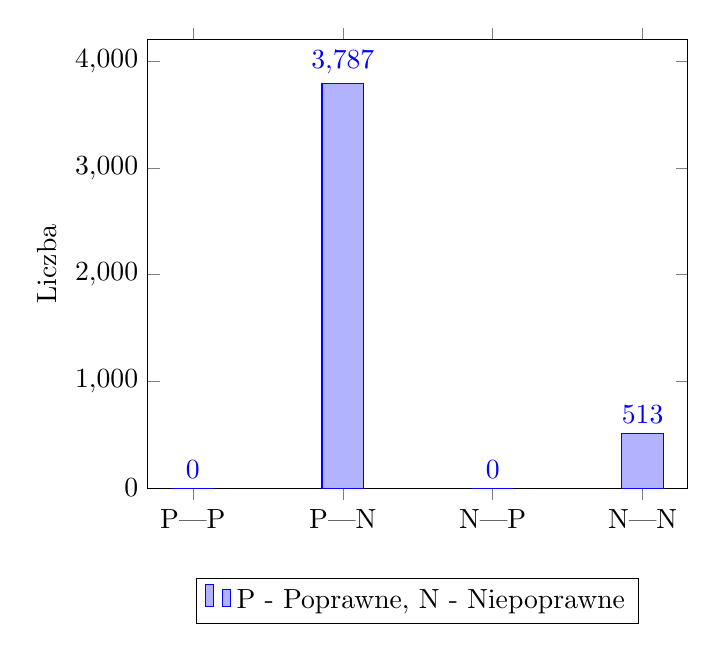
\begin{tikzpicture}
\begin{axis}[
    ybar,
    symbolic x coords={P|P, P|N, N|P, N|N},
    xtick=data,
    ylabel={Liczba},
    nodes near coords,
    bar width=15pt,
    legend style={at={(0.5,-0.20)}, anchor=north, legend columns=-1},
    ymin=0,
    ymax=4200,
]
\addplot coordinates {(P|P,0) (P|N,3787) (N|P,0) (N|N,513)};
\addlegendentry{P - Poprawne, N - Niepoprawne}
\end{axis}
\end{tikzpicture}
\caption{Wykres wyników sprawdzenia poprawności dla zbioru testowego przy zastosowaniu kontrolnego DMJ oraz generatora kodu.}\label{rys:plama2k}
\end{figure}

Dla lepszej wizualizacji wyników zestawiono liczbowo wartości modeli sklasyfikowanych jako \textbf{poprawne} dla generatora \akronim{ZIMPL} oraz kontrolnego DMJ. Wartość \( z \) przedstawiona w poniższej tablicy~\ref{tab:experiment:analysis4} wynosi -82,26 zatem różnica jest statystycznie istotna.

\begin{table}[H]
\caption{Estymacja przedziału ufności wraz z testem z}\label{tab:experiment:analysis4}
\centering%
\begin{tabular}{|l|c|c|}
\hline
\textbf{Kategoria} & \textbf{Generator} & \textbf{Kontrolny DMJ} \\
\hline
\textbf{Liczba modeli ($n$)} & 4300 & 4300 \\
\hline
\textbf{Poprawne modele ($m$)} & 3787 & 0 \\
\hline
\textbf{Proporcja (\%)} & 88,07 & 0,00 \\
\hline
\textbf{Przedział ufności (95\%)} & [87,10 ; 89,04] & [0,00 ; 0,00] \\
\hline
\multicolumn{3}{|c|}{Wartość statystyki \( z \): -82,26} \\
\hline
\end{tabular}
\end{table}

\section{Jak dużą poprawę jakości składni uzyskuje generator względem kontrolnego DMJ?}
% TP: TODO: sugeruję zmienić na "Jak dużą poprawę jakości składni uzyskuje generator względem kontrolnego DMJ?" i dalej pisać o kontrolnym DMJ - DONE

Dla modeli PL w formule sztywnej generator uzyskał \textbf{3,31p}, a kontrolny DMJ \textbf{1,81p} na 4-punktowej skali jakości zdefiniowanej poniżej. Dla modeli PL w formule parametryzowanej, generator uzyskał \textbf{4,75p}, a kontrolny DMJ \textbf{2,78p} na 6-punktowej skali jakości zdefiniowanej poniżej.

% TP: TODO: tutaj wypadałoby zrobić 2 testy statystyczne na różnice generator vs kontrolny DMJ; ta skala punktowa jest arbitralna, więc rozkład wartości może być nietypowy i byłbym ostrożny w stosowaniu testów parametrycznych; raczej sugeruję użyć np. Wilcoxona dla alpha=0,05 https://pl.wikipedia.org/wiki/Test_Wilcoxona_dla_par_obserwacji

Do sprawdzenia jakości modelu PL pod względem jego składni i jakości zrozumienia zadania zastosowano ocenę ekspercką, w~której ekspert przyznawał punkty dla czterech (formuła sztywna) lub sześciu (formuła parametryzowana) kryteriów. W~roli eksperta wykorzystano DMJ \textit{GPT-4o} \cite{TODO}, który jest niezależny od DMJ stosowanych w generatorze i kontrolnym DMJ. Po otrzymaniu wyników, dla większej wiarygodności, wykonano oczyszczanie rezultatów i naprawę oczywistych błędów halucynowanych przez DMJ. % TP: TODO <- opiszcie dokładnie procedurę czyszczenia i naprawy; jak dobrze rozumiem, w Sekcji 5.4 nie było takiej procedury; gdyby jednak była też tam stosowana, to wtedy możecie to czyszczenie dodać do opisu kontrolengo DMJ z sekcji 5.1
% TP: TODO: tutaj brakuje też dokładnego udokumentowania procedury odpytania DMJ, tzn. jakiego prompta dostał? Czy to była sekwencja pytań i odpowiedzi? itd. Jako, że prompty są pewnie dedykowane pod formułę poniżej, to możecie je pokazać w poniższych sekcjach.

%Zależnie od funkcjonalności kodu, wykorzystano inne mierniki jakości. Dla wyników parametryzowanych zastosowano skalę sześciostopniową, podczas gdy dla sztywnego kodowania - czterostopniową.

%Wynikiem eksperymentu jest punktacja \textbf{3,31/4,00} dla wygenerowanych wyników, w porównaniu do \textbf{1,81/4,00} dla standardowego zapytania, dla wszystkich wyników sztywnego kodowania. Tak samo, dla parametryzowanych wyników powstałych w wyniku wykorzystania generatora oceną jest \textbf{4,75/6,00}, podczas gdy dla pojedynczego zapytania wynosi \textbf{2,78/6,00}. Sumaryczna poprawa względem standardowego zapytania \textbf{wzrosła o średnio 1,74} punktu.

\subsection{Modele PL w sztywnej formule.}

Dla wynikowych modeli PL w \textbf{sztywnej formule} poddano ocenie poniższe kryteria binarne w odniesieniu do wzorcowego modelu PL zawartego w danych testowych:

\begin{enumerate}
\item \textbf{Definiowanie zmiennych} -- $1$p jeśli wszystkie zmienne i ich typy są zgodne z modelem wzorcowym. Nazwy zmiennych i komentarze mogą się różnić, ale logika ich wykorzystania musi pozostać taka sama. Niespełnienie tego wymagania powoduje przyznanie $0$p. % TP: <- zmieniłem, zweryfikujcie; czy jeśli generator _zadeklaruje_ wiecej zmiennych niż potrzeba, ale dobrze użyje tylko części zmiennych to dostanie punkt czy nie?
\item \textbf{Funkcja celu} -- $1$p jeśli funkcja celu jest semantycznie równa funkcji celu w modelu wzorcowym, łącznie z kierunkiem optymalizacji. Semantyczna równość to równość algebraiczną po uzgodneniu mapowania między nazwami zmiennych w obu modelach. Nazwy funkcji i zmiennych nie mają znaczenia. Funkcje niezgodne semantycznie skutkują przyznaniem $0$p.
\item \textbf{Ograniczenia} -- aby otrzymać $1$p, ograniczenia muszą być zdefiniowane zgodnie ze wzorcowym modelem. Liczba, logika i zapis muszą być zgodne, a każde ograniczenie powinno zaczynać się od \texttt{subto <nazwa>:}. Zastosowanie innej struktury powoduje przyznanie $0$p.
\item \textbf{Inne wymagania} -- $1$p przyznaje się za spełnienie wymagań takich jak: użycie \texttt{\#} jako prefiksu komentarzy, brak zbędnych poleceń oraz poprawne rozpoczęcie każdej linii od jednego z kluczowych słów (\texttt{var}, \texttt{minimize}, \texttt{maximize}, \texttt{subto}). % TP: TODO: To trzeba doprecyzować - czy tutaj każdy czynnik jest oceniany 0,25p i razem sumuje się do 1p? Czy jeśli jeden komentarzb będzie zaczynać się od \#, a drugi nie to punkt zostanie przyznany? Czy puste linie dyskwalifikują przyznanie punktu? Czy długie ograniczenie rozpisane na wiele linii dyskwalifikuje przyznanie punktu?
\end{enumerate}

Poniżej przedstawiona została analiza wyników generatora oraz kontrolnego DMJ dla poszczególnych kategorii.

\begin{table}[H]
\caption{Tabela ocenionych wyników dla kategorii \textbf{Definiowanie zmiennych}.}\label{tab:tabela12}
\centering%
\begin{tabular}{|l|c|c|}
\hline
\textbf{Punktacja} & \textbf{Generator} & \textbf{Kontrolny DMJ}\\
\hline
1 & 1832 & 1418 \\
\hline
0 & 443 & 857 \\
\hline
Średnia ocena & 0,81 & 0,62 \\
\hline
\end{tabular}
\end{table}

% TP: TODO: test statystyczny na różnice średnich/frakcje dla \alpha=0,05, np. https://pl.wikipedia.org/wiki/Test_dla_proporcji#Test_dla_dwóch_prób_dużych

Już pierwszy wynik pokazuje większą skuteczność generatora ponad pojedynczym zapytaniem. Podstawowym błędem popełnianym w deklaracji zmiennych jest niezgodna w porównaniu z zadaniem ich liczba. % TP: TODO: za dużo? za mało? nieadekwatne zmienne? Macie na to jakieś statystyki do pokazania?

\begin{table}[H]
\caption{Tabela ocenionych wyników dla kategorii \textbf{Funkcja celu}.}\label{tab:tabela13}
\centering%
\begin{tabular}{|l|c|c|}
\hline
\textbf{Punktacja} & \textbf{Generator} & \textbf{Kontrolny DMJ}\\
\hline
1 & 1882 & 1469 \\
\hline
0 & 393 & 806 \\
\hline
Średnia ocena & 0,83 & 0,65 \\
\hline
\end{tabular}
\end{table}

% TP: TODO: test statystyczny jw.

Generator tworzy poprawne funkcje celu %TP: TODO: zależnie od wyników testu statystycznego: jeśli wyjdzie różnica to "znacząco", jeśli brak różnicy to "nieznacznie"
częściej od kontrolnego DMJ. 
Znacznie większe różnice zachodzą dla ograniczeń. Kontrolny DMJ w każdym z przypadków testowych generuje kod zwierający w sobie niepoprawną deklarację ograniczenia, przez co nigdy nie został sklasyfikowany jako poprawny. % TP: TODO: w tabeli jednak widać, że zdobywa jedyniki - chyba błąd w danych; zobaczcie, że średnie też nie pasują do danych.

\begin{table}[H]
\caption{Tabela ocenionych wyników dla kategorii \textbf{Ograniczenia}.}\label{tab:tabela14}
\centering%
\begin{tabular}{|l|c|c|}
\hline
\textbf{Punktacja} & \textbf{Generator} & \textbf{Kontrolny DMJ}\\
\hline
1 & 2140 & 1754 \\
\hline
0 & 0 & 2275 \\
\hline
Średnia ocena & 0,94 & 0,00 \\
\hline
\end{tabular}
\end{table}

% TP: TODO: test statystyczy jw.

Największą trudnością dla obu DMJ jest uzyskanie pozytywnej punktacji w kategorii \textbf{Inne wymagania}. Wpływa na to fakt, iż jest to kategoria sprawdzająca wszystkie, wcześniej nieuwzględnione błędy, a zatem łatwo w niej stracić punkt. Również w tym przypadku generator okazał się nieco lepszy.

\begin{table}[H]
\caption{Tabela ocenionych wyników dla kategorii \textbf{Inne wymagania}.}\label{tab:tabela15}
\centering%
\begin{tabular}{|l|c|c|}
\hline
\textbf{Punktacja} & \textbf{Generator} & \textbf{Kontrolny DMJ}\\
\hline
1 & 1665 & 1229 \\
\hline
0 & 610 & 1046 \\
\hline
Średnia ocena & 0,73 & 0,54 \\
\hline
\end{tabular}
\end{table}

% TP: TODO: test statystyczny

% TP: TODO: sugeruje to przenieść na początek 5.5; tzn. zintegrować z tamtym tekstem i umieścić tam tabele 5.15 oraz wykresy
Wyniki zapewnianie dla sztywnego formułowania modeli  \textit{ZIMPL} zapewniają poprawę, ale nie jest ona tak wysoka, jak przy parametryzowanych danych. W średnio wyniki otrzymują ocenę w 3,31, podczas gdy dla kontrolnego DMJ ten wynik zmniejsza się o 1,50 punktu (średnio 1,81).

\begin{table}[H]
\caption{Tabela sumarycznej oceny wyników dla kodowanych sztywno modeli.}\label{tab:tabela16}
\centering%
\begin{tabular}{|l|c|c|}
\hline
\textbf{Punktacja} & \textbf{Generator} & \textbf{Kontrolny DMJ}\\
\hline
0 & 103 & 509 \\
\hline
1 & 46 & 442 \\
\hline
2 & 386 & 298 \\
\hline
3 & 259 & 1026 \\
\hline
4 & 1481 & 0 \\
\hline
\textbf{Średnia ocena} & \textbf{3,31} & \textbf{1,81} \\
\hline
\end{tabular}
\end{table}

\begin{figure}[H]
\centering
\begin{minipage}{0.45\textwidth}
\centering
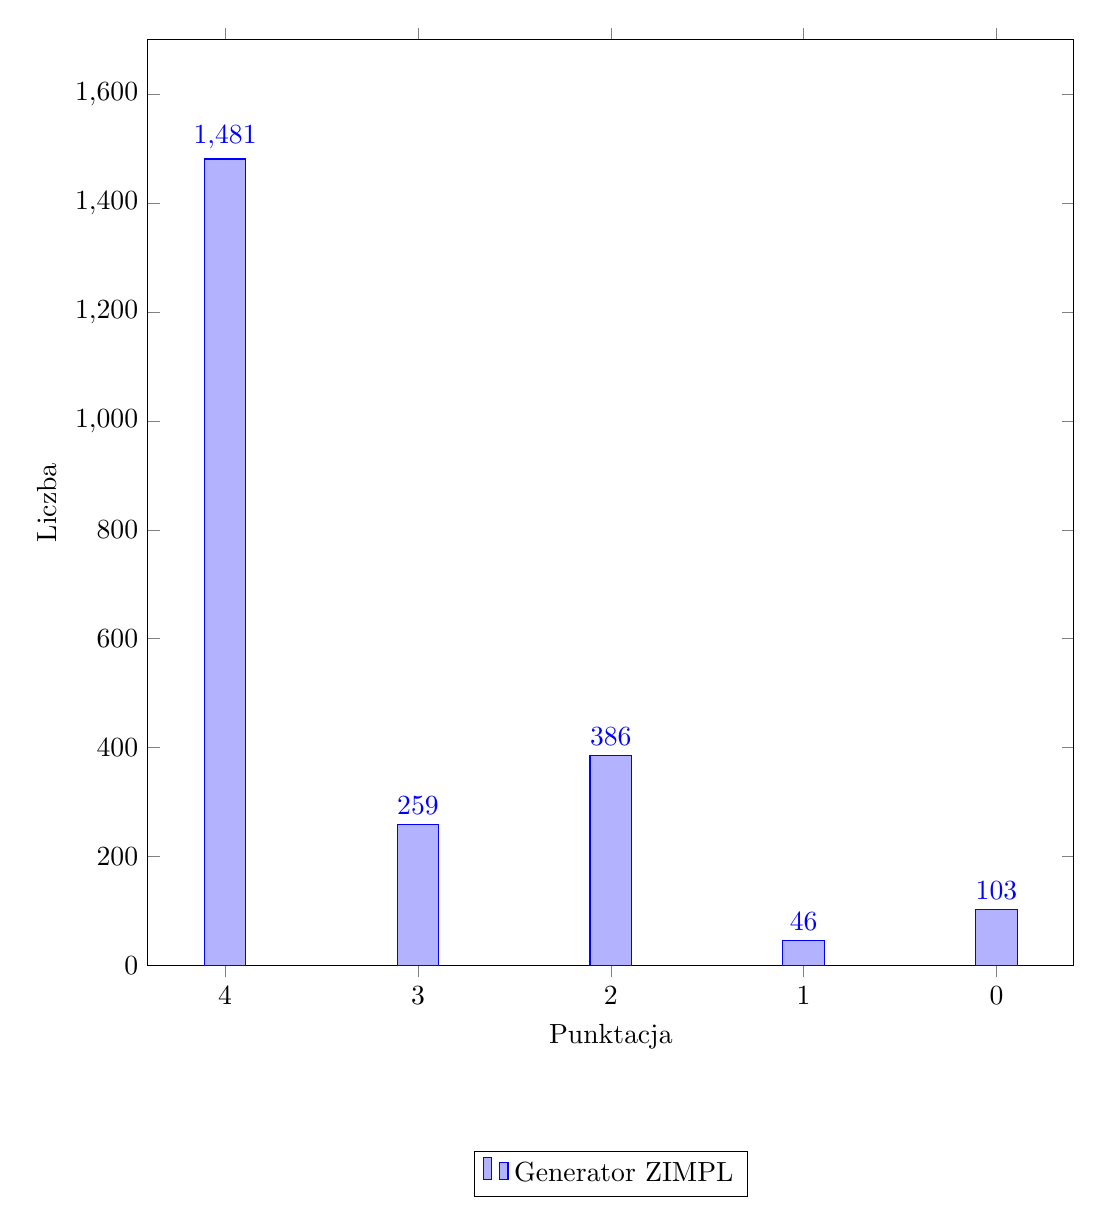
\begin{tikzpicture}
\begin{axis}[
    ybar,
    symbolic x coords={4,3,2,1,0},
    xtick=data,
    ylabel={Liczba},
    width=1.1\textwidth,
    height=1.1\textwidth,
    nodes near coords,
    bar width=15pt,
    ymin=0,
    ymax=1700,
    xlabel={Punktacja},
    legend style={at={(0.5,-0.20)}, anchor=north, legend columns=-1}
]
\addplot coordinates {(4,1481) (3,259) (2,386) (1,46) (0,103)};
\addlegendentry{Generator ZIMPL}
\end{axis}
\end{tikzpicture}
\end{minipage}%
\hspace{0.05\textwidth}
\begin{minipage}{0.45\textwidth}
\centering
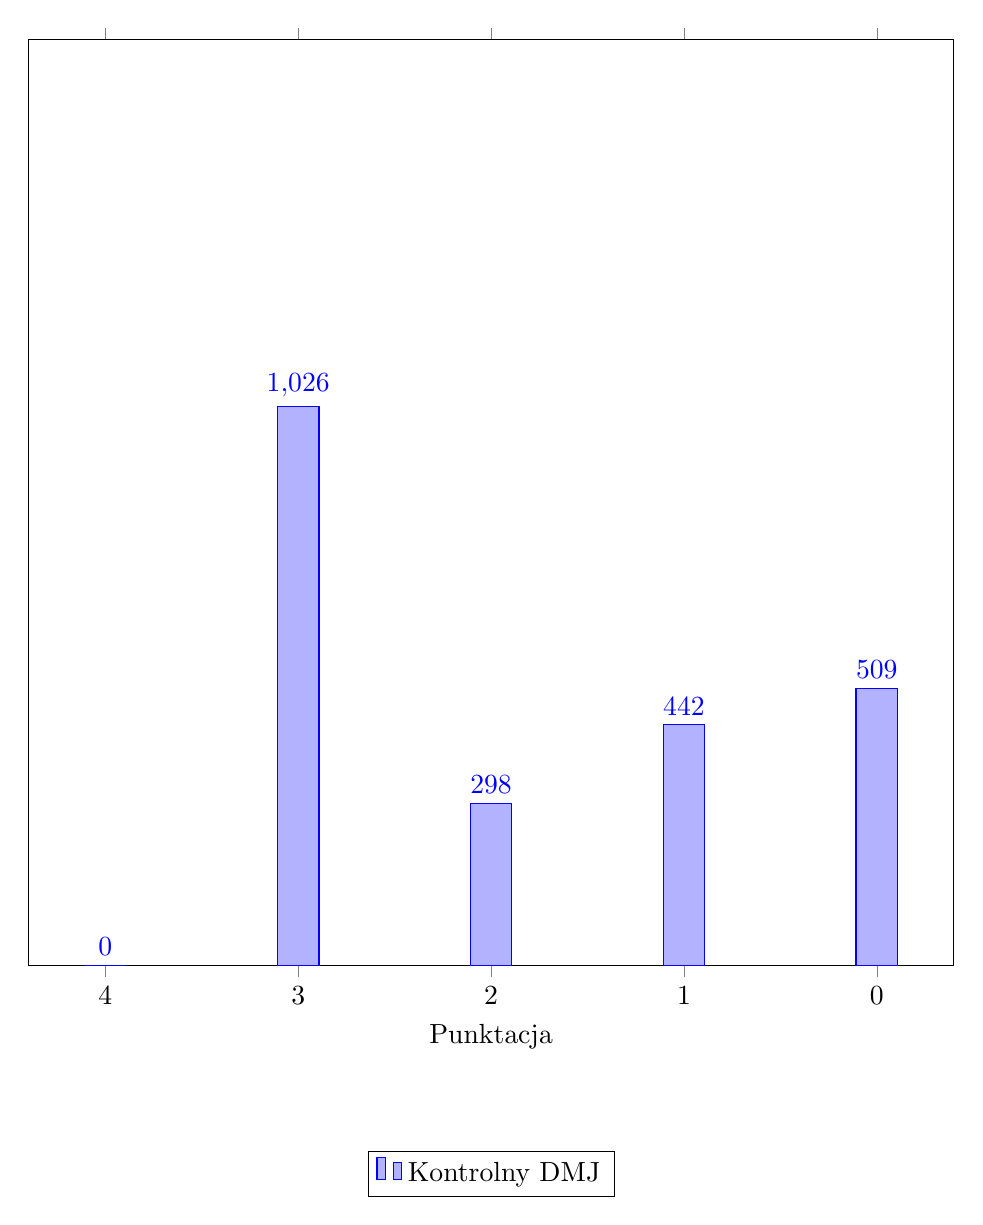
\begin{tikzpicture}
\begin{axis}[
    ybar,
    symbolic x coords={4,3,2,1,0},
    xtick=data,
    %ylabel={Liczba},
    width=1.1\textwidth,
    height=1.1\textwidth,
    ytick = \empty,
    nodes near coords,
    bar width=15pt,
    ymin=0,
    ymax=1700,
    xlabel={Punktacja},
    legend style={at={(0.5,-0.20)}, anchor=north, legend columns=-1}
]
\addplot coordinates {(4,0) (3,1026) (2,298) (1,442) (0,509)};
\addlegendentry{Kontrolny DMJ}
\end{axis}
\end{tikzpicture}
\end{minipage}
\caption{Wykres prezentujący sumaryczną ocenę wyników dla parametryzowanych modeli.} % TP: TODO: ...dla modeli w sztywnej formule?
\end{figure}

\subsection{Modele PL w parametryzowanej formule.}

Dla wynikowych modeli PL w \textbf{formule parametryzowanej} poddano ocenie poniższe kryteria binarne w~odniesieniu do wzorcowych modeli PL zawartych w danych testowych: 
%Podobna analiza została przeprowadzona dla modeli parametryzowanych. Dla kategorii, jakie przedstawiają, przewaga generatora jest znacznie wyższa. Wynika to z złożoności kodu, z jakim pracuje. Modele generowane za pomocą pojedynczego zapytania nie posiadają wiedzy na temat struktury kodu, przez co mają problemy z identyfikacją zbiorów i parametrów. Punktacja w tym przypadku jest w kategoriach:

\begin{enumerate}
\item \textbf{Definiowanie zbiorów} -- $1$p jeśli wszystkie zbiory są poprawnie zdefiniowane przy użyciu nawiasów klamrowych \texttt{{}}, z elementami w cudzysłowach. % TP: TODO: a jeśli wartościami zbioru są liczby?
 Każde odstępstwo od składni, powoduje utratę punktu. % TP: TODO: czy nie ma tutaj weryfikacji semantycznej? Wcześniejsze kryteria to uwzględniały
 W przeciwnym wypadku $0$p.
\item \textbf{Definiowanie parametrów} -- $1$p jeśli wszystkie parametry są poprawnie zindeksowane za pomocą nawiasów kwadratowych \texttt{[ ]} % TP: TODO: co jeśli wzorcowy parametr jest skalarem, a nie wektorem?
i logicznie zgodne z poprawnym kodem. % TP: TODO: co to dokładnie znaczy, że są logicznie zgodne?
Nazwy parametrów mogą się różnić, o ile zachowano ich poprawne zastosowanie. W przeciwnym wypadku $0$p.
\item \textbf{Definiowanie zmiennych} -- $1$p jeśli wszystkie zmienne i ich typy % TP: TODO: dziedziny?
są zgodne z modelem wzorcowym. Zmienne muszą być indeksowane odpowiednimi zbiorami. Nazwy zmiennych i komentarze mogą się od różnić, ale logika ich wykorzystania musi pozostać taka sama. Brak zgodności powoduje przyznanie $0$p.
\item \textbf{Funkcja celu} -- $1$p jeśli funkcja celu jest semantycznie równa funkcji celu w modelu wzorcowym, łącznie z kierunkiem optymalizacji. Semantyczna równość to równość algebraiczną po uzgodneniu mapowania między nazwami zmiennych w obu modelach. Nazwy funkcji i zmiennych nie mają znaczenia. Funkcje niezgodne semantycznie skutkują przyznaniem $0$p.
\item \textbf{Ograniczenia} -- aby otrzymać $1$p, ograniczenia muszą być zdefiniowane zgodnie ze wzorcowym modelem. Liczba, logika i zapis muszą być zgodne, a każde ograniczenie powinno zaczynać się od \texttt{subto <nazwa>:}. Zastosowanie innej struktury powoduje przyznanie $0$p.
\item \textbf{Inne wymagania} -- $1$p przyznaje się za spełnienie wymagań takich jak: użycie \texttt{\#} jako prefiksu komentarzy, brak zbędnych poleceń oraz poprawne rozpoczęcie każdej linii od jednego z kluczowych słów (\texttt{var}, \texttt{minimize}, \texttt{maximize}, \texttt{subto}). % TP: TODO: To trzeba doprecyzować - czy tutaj każdy czynnik jest oceniany 0,25p i razem sumuje się do 1p? Czy jeśli jeden komentarzb będzie zaczynać się od \#, a drugi nie to punkt zostanie przyznany? Czy puste linie dyskwalifikują przyznanie punktu? Czy długie ograniczenie rozpisane na wiele linii dyskwalifikuje przyznanie punktu?
\end{enumerate}

% TP: TODO: poprawcie proszę niżej analogicznie do sekcji 5.5.1 -> ja kontynuuję sprawdzanie w Rozdziale 6

Już w pierwszej kategorii widać znaczącą różnicę w wynikach między generowanymi wynikami. Kontrolny DMJ nie radzi sobie z tworzeniem zbiorów, stosując błędną implementację. Średnie wyniki uzyskanej punktacji różnią się od siebie o \textbf{0,33} punktu, co jest najwyższym dotąd uzyskanym wynikiem.

\begin{table}[H]
\caption{Tabela ocenionych wyników dla kategorii \textbf{Definiowanie zbiorów}.}\label{tab:tabela17}
\centering%
\begin{tabular}{|l|c|c|}
\hline
\textbf{Punktacja} & \textbf{Generator} & \textbf{Kontrolny DMJ}\\
\hline
1 & 1783 & 914 \\
\hline
0 & 242 & 1111 \\
\hline
Średnia ocena & 0,88 & 0,45 \\
\hline
\end{tabular}
\end{table}

Tworzenie parametrów prezentuje znacznie lepsze wyniki, zapewniając prawie 100\% skuteczności w tworzeniu przez generator. Wyniki kontrolnego DMJ również utrzymują się na poziomie powyżej 80\%.

\begin{table}[H]
\caption{Tabela ocenionych wyników dla kategorii \textbf{Definiowanie parametrów}.}\label{tab:tabela18}
\centering%
\begin{tabular}{|l|c|c|}
\hline
\textbf{Punktacja} & \textbf{Generator} & \textbf{Kontrolny DMJ}\\
\hline
1 & 2008 & 1663 \\
\hline
0 & 17 & 362 \\
\hline
Średnia ocena & 0,99 & 0,82 \\
\hline
\end{tabular}
\end{table}

Definiowanie zmiennych na podstawie zbiorów i parametrów obniża jakość wyniku kodu, przez co nie zostaje osiągnięta 100\% poprawność, tak jak w przypadku sztywnego formatu kodu. Wyniki generatora w tym przypadku są nieznacznie wyższe.

\begin{table}[H]
\caption{Tabela ocenionych wyników dla kategorii \textbf{Definiowanie zmiennnych}.}\label{tab:tabela19}
\centering%
\begin{tabular}{|l|c|c|}
\hline
\textbf{Punktacja} & \textbf{Generator} & \textbf{Kontrolny DMJ}\\
\hline
1 & 1713 & 1473 \\
\hline
0 & 312 & 552 \\
\hline
Średnia ocena & 0,85 & 0,73 \\
\hline
\end{tabular}
\end{table}


Generowanie funkcji celu na podstawie wcześniej zdeklarowanych zmiennych działa bardzo dobrze, a wyniki posiadają poprawnie zdefiniowaną minimalizację/maksymalizację, a także prawidłowe sumowanie na zbiorach.

\begin{table}[H]
\caption{Tabela ocenionych wyników dla kategorii \textbf{Funkcja celu}.}\label{tab:tabela20}
\centering%
\begin{tabular}{|l|c|c|}
\hline
\textbf{Punktacja} & \textbf{Generator} & \textbf{Kontrolny DMJ}\\
\hline
1 & 2002 & 2000 \\
\hline
0 & 23 & 25 \\
\hline
Średnia ocena & 0,83 & 0,65 \\
\hline
\end{tabular}
\end{table}

Znacząca różnica pojawia się przy porównywaniu ograniczeń. Kontrolny DMJ nie zna składni kodu  \textit{ZIMPL}, w związku z czym każdorazowo deklaruje niepoprawne ograniczenia, używając takich elementów jak \texttt{s.t.} lub \texttt{subject to}.

\begin{table}[H]
\caption{Tabela ocenionych wyników dla kategorii \textbf{Ograniczenia}.}\label{tab:tabela21}
\centering%
\begin{tabular}{|l|c|c|}
\hline
\textbf{Punktacja} & \textbf{Generator} & \textbf{Kontrolny DMJ}\\
\hline
1 & 1790 & 0 \\
\hline
0 & 235 & 2025 \\
\hline
Średnia ocena & 0,88 & 0,00 \\
\hline
\end{tabular}
\end{table}


W przypadku ostatniej z ocenianych kategorii, modele osiągnęły niskie oceny. Wynikało to ponownie z ogólności kategorii. Wszelkie błędy, które nie zostały wyłapane w pozostałych kategoriach, zostały rozliczone w tym miejscu. Modele  \textit{ZIMPL} straciły najwięcej punktów na tworzeniu niepotrzebnych i niezwiązanych z problemem komend. 

\begin{table}[H]
\caption{Tabela ocenionych wyników dla kategorii \textbf{Inne wymagania}.}\label{tab:tabela22}
\centering%
\begin{tabular}{|l|c|c|}
\hline
\textbf{Punktacja} & \textbf{Generator} & \textbf{Kontrolny DMJ}\\
\hline
1 & 658 & 259 \\
\hline
0 & 1367 & 1766 \\
\hline
Średnia ocena & 0,32 & 0,13 \\
\hline
\end{tabular}
\end{table}


W poniższym zestawieniu sumarycznych rezultatów widać, że stworzony generator kodu  \textit{ZIMPL} został znacznie lepiej oceniony, niż kontrolny DMJ. W większości wypadków utrzymuje on wynik w okolicy 5 punktów (średnio 4,75), co świadczy o wysokiej jakości. Ta różnica jest znacząca w porównaniu do wyniku kontrolnego DMJ, który jest niższy o 1,97 punktu utrzymując średni poziom 2,78 punktu.

\begin{table}[H]
\caption{Tabela sumarycznej oceny wyników dla parametryzowanych modeli.}\label{tab:tabela23}
\centering%
\begin{tabular}{|l|c|c|}
\hline
\textbf{Punktacja} & \textbf{Generator} & \textbf{Kontrolny DMJ}\\
\hline
0 & 3 & 3 \\
\hline
1 & 1 & 80 \\
\hline
2 & 23 & 464 \\
\hline
3 & 293 & 650 \\
\hline
4 & 61 & 789 \\
\hline
5 & 1080 & 39 \\
\hline
6 & 564 & 0 \\
\hline
\textbf{Średnia ocena} & \textbf{4,75} & \textbf{2,78} \\
\hline
\end{tabular}
\end{table}

\begin{figure}[H]
\centering
\begin{minipage}{0.45\textwidth}
\centering
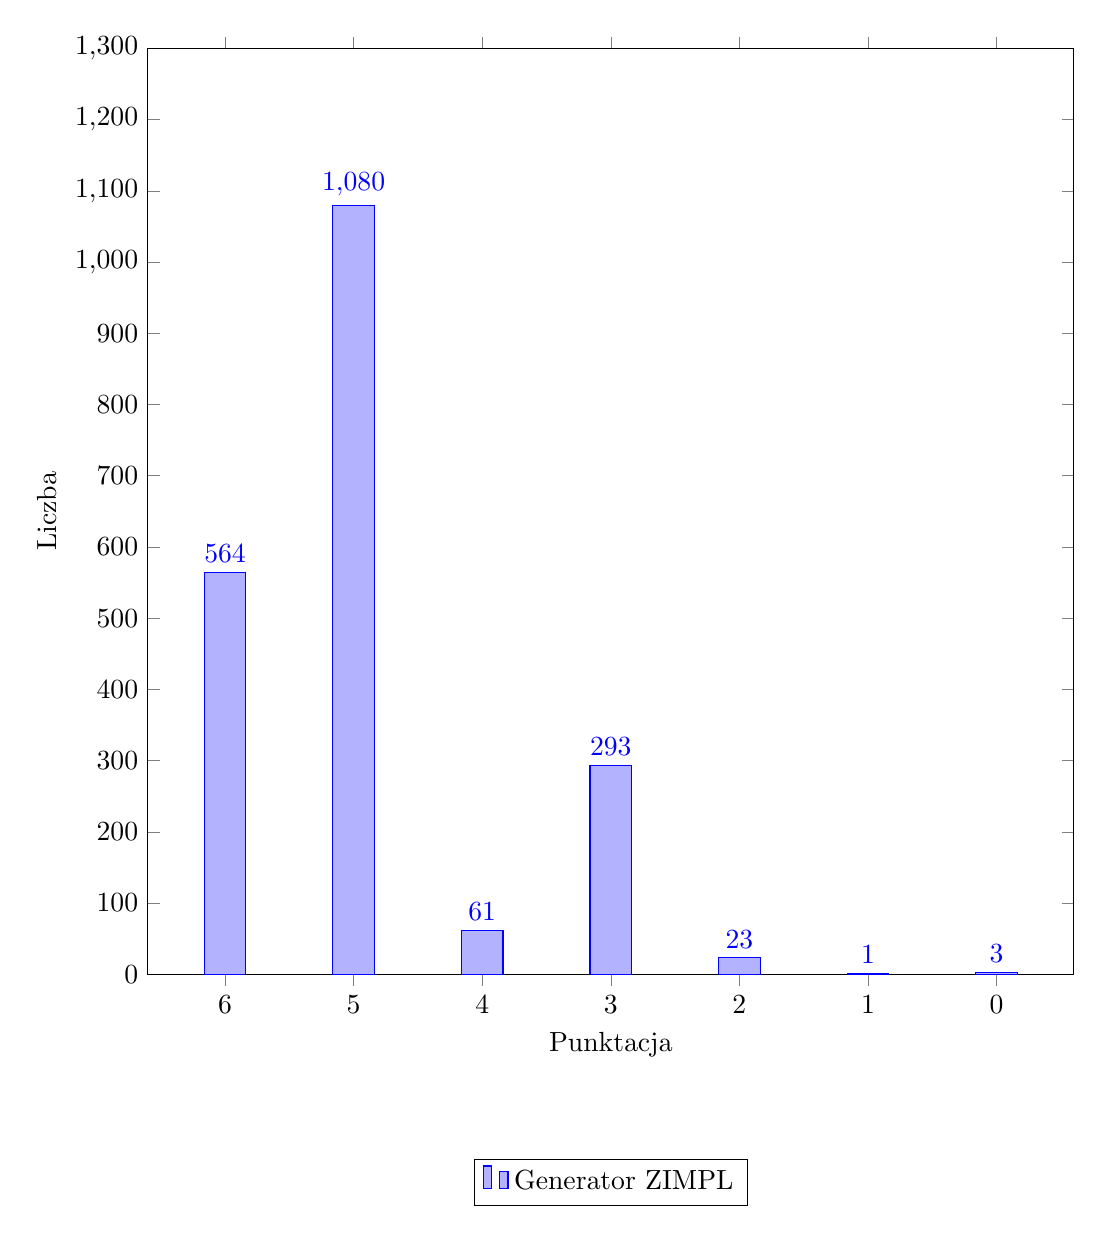
\begin{tikzpicture}
\begin{axis}[
    ybar,
    symbolic x coords={6,5,4,3,2,1,0},
    xtick=data,
    ylabel={Liczba},
    width=1.1\textwidth,
    height=1.1\textwidth,
    nodes near coords,
    bar width=15pt,
    ymin=0,
    ymax=1300,
    xlabel={Punktacja},
    legend style={at={(0.5,-0.20)}, anchor=north, legend columns=-1}
]
\addplot coordinates {(6,564) (5,1080) (4,61) (3,293) (2,23) (1,1) (0,3)};
\addlegendentry{Generator ZIMPL}
\end{axis}
\end{tikzpicture}
\end{minipage}%
\hspace{0.05\textwidth}
\begin{minipage}{0.45\textwidth}
\centering
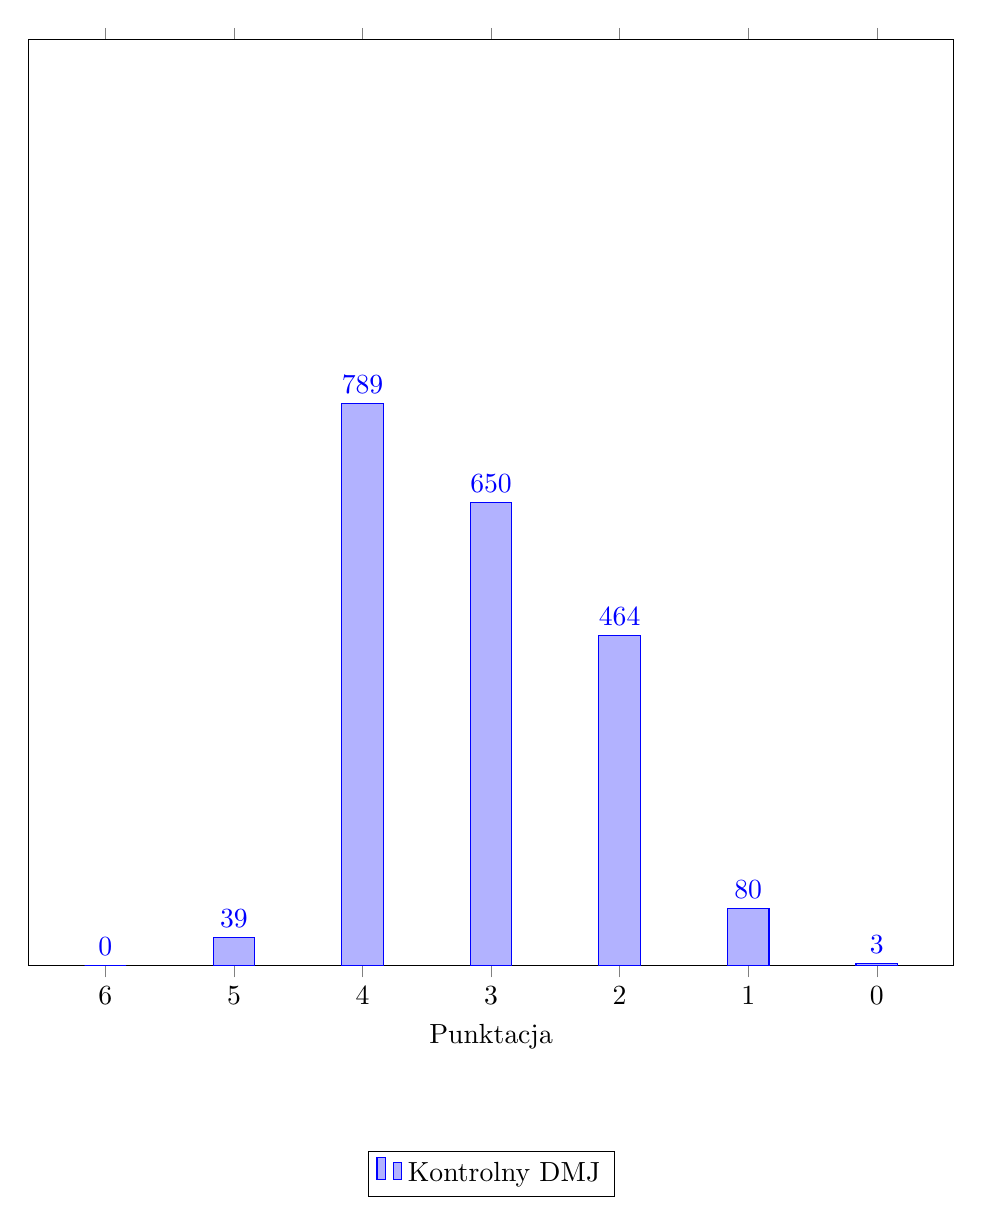
\begin{tikzpicture}
\begin{axis}[
    ybar,
    symbolic x coords={6,5,4,3,2,1,0},
    xtick=data,
    %ylabel={Liczba},
    width=1.1\textwidth,
    height=1.1\textwidth,
    ytick = \empty,
    nodes near coords,
    bar width=15pt,
    ymin=0,
    ymax=1300,
    xlabel={Punktacja},
    legend style={at={(0.5,-0.20)}, anchor=north, legend columns=-1}
]
\addplot coordinates {(6,0) (5,39) (4,789) (3,650) (2,464) (1,80) (0,3)};
\addlegendentry{Kontrolny DMJ}
\end{axis}
\end{tikzpicture}
\end{minipage}
\caption{Wykres prezentujący sumaryczną ocenę wyników dla parametryzowanych modeli.}
\end{figure}

\chapter{Dyskusja} %1.5-2 strony

Spojrzeć na rozwiązanie wysokopoziomowe, co jest dobre, co jest złe, co można poprawić (postawić hipotezy jak postawić), dlaczego pewnych rzeczy nie da się zrobić (np. duże problemy PL, ograniczenia językowe, etc), odnieść się do innych projektów – co nam nie pomogło, co pomogło, czemu wykorzystaliśmy dane rzeczy




\chapter{Wnioski i dalszy kierunek prac}\label{ch:conclusions}

\section{Wnioski}
Na początku pracy postawiono hipotezę badawczą:
\begin{quote}
\textit{Można wykorzystać duże modele językowe do generowania modeli PL zapisanych w języku naturalnym.}
\end{quote}

Analizując przedstawione rozwiązanie i wspomagając się eksperymentami założono poprawność powyższej hipotezy. Przy odpowiednio przygotowanym zapytaniu można z dużą pewnością założyć, że duże modele językowe można wykorzystać do generowania modeli PL otrzymując na wejściu jedynie problem zapisany w języku naturalnym. Istnieje znacząca poprawa w jakości wygenerowanego rozwiązania w stosunku do rozwiązania za pomocą pojedynczego, prostego zapytania. Zaobserwowano wzrost skuteczności dużych modeli językowych przy generowaniu modeli \textit{PL}. Przekłada się to na usprawnienie procesu modelowania optymalizacyjnego. 

Wyniki eksperymentu pokazały, iż bardziej precyzyjne oraz szczegółowo sformułowane zapytania, przekładają się bezpośrednio na wzrost jakości wygenerowanego modelu \textit{PL} przez \textit{DMJ}. Redukuje to konieczność kosztownej w zasobach i czasie pracy ekspertów. Rozwiązanie to zmniejsza liczbę błędów oraz redukuje niedoskonałości wykonania wynikające z czynnika ludzkiego. 

Zauważono również, iż zwiększenie różnorodności przykładów przyczyniłoby się do poprawy jakości generowanych modeli \textit{PL} przez duże modele językowe. Tworzy to dodatkowe adaptacje dla dużych modeli językowych oraz polepsza ich elastyczność.

\section{Dalszy kierunek prac}

Kolejnym etapem rozwoju sytemu generującego modele \textit{PL} byłoby wzbogacenie bazy danych o bardziej różnorodne przykłady. Dodanie większej ilości niestandardowych problemów może istotnie poprawić jakość generowanych rozwiązań.

Istotnym rozważenia jest również adaptacja alternatywnych narzędzi typu \textit{solver} takich jak \textit{Gurobi}. Poszerzyłoby to horyzonty w implementacji użytego rozwiązania na nowe obszary dziedziny optymalizacji. Istnieje również możliwość opracowania narzędzi do wizualizacji, pozwalających na graficzną reprezentację problemów \textit{PL}, co ułatwiłoby odbiór oraz interpretacje wygenerowanego rozwiązania. 

Skoncentrowanie się na poszerzeniu zakresu zbioru danych, również może zwiększyć dokładność generowanych modeli \textit{PL} przez \textit{DMJ}. 

%--------------------------------------
% Literatura
%--------------------------------------

\bibliographystyle{plain}{\raggedright\sloppy\small\bibliography{bibliografia}}


%--------------------------------------
% Informacja o prawach autorskich
%--------------------------------------

\ppcolophon

\end{document}
